\batchmode
\documentclass[twoside]{book}

% Packages required by doxygen
\usepackage{fixltx2e}
\usepackage{calc}
\usepackage{doxygen}
\usepackage[export]{adjustbox} % also loads graphicx
\usepackage{graphicx}
\usepackage[utf8]{inputenc}
\usepackage{makeidx}
\usepackage{multicol}
\usepackage{multirow}
\PassOptionsToPackage{warn}{textcomp}
\usepackage{textcomp}
\usepackage[nointegrals]{wasysym}
\usepackage[table]{xcolor}

% Font selection
\usepackage[T1]{fontenc}
\usepackage[scaled=.90]{helvet}
\usepackage{courier}
\usepackage{amssymb}
\usepackage{sectsty}
\renewcommand{\familydefault}{\sfdefault}
\allsectionsfont{%
  \fontseries{bc}\selectfont%
  \color{darkgray}%
}
\renewcommand{\DoxyLabelFont}{%
  \fontseries{bc}\selectfont%
  \color{darkgray}%
}
\newcommand{\+}{\discretionary{\mbox{\scriptsize$\hookleftarrow$}}{}{}}

% Page & text layout
\usepackage{geometry}
\geometry{%
  a4paper,%
  top=2.5cm,%
  bottom=2.5cm,%
  left=2.5cm,%
  right=2.5cm%
}
\tolerance=750
\hfuzz=15pt
\hbadness=750
\setlength{\emergencystretch}{15pt}
\setlength{\parindent}{0cm}
\setlength{\parskip}{3ex plus 2ex minus 2ex}
\makeatletter
\renewcommand{\paragraph}{%
  \@startsection{paragraph}{4}{0ex}{-1.0ex}{1.0ex}{%
    \normalfont\normalsize\bfseries\SS@parafont%
  }%
}
\renewcommand{\subparagraph}{%
  \@startsection{subparagraph}{5}{0ex}{-1.0ex}{1.0ex}{%
    \normalfont\normalsize\bfseries\SS@subparafont%
  }%
}
\makeatother

% Headers & footers
\usepackage{fancyhdr}
\pagestyle{fancyplain}
\fancyhead[LE]{\fancyplain{}{\bfseries\thepage}}
\fancyhead[CE]{\fancyplain{}{}}
\fancyhead[RE]{\fancyplain{}{\bfseries\leftmark}}
\fancyhead[LO]{\fancyplain{}{\bfseries\rightmark}}
\fancyhead[CO]{\fancyplain{}{}}
\fancyhead[RO]{\fancyplain{}{\bfseries\thepage}}
\fancyfoot[LE]{\fancyplain{}{}}
\fancyfoot[CE]{\fancyplain{}{}}
\fancyfoot[RE]{\fancyplain{}{\bfseries\scriptsize Generated by Doxygen }}
\fancyfoot[LO]{\fancyplain{}{\bfseries\scriptsize Generated by Doxygen }}
\fancyfoot[CO]{\fancyplain{}{}}
\fancyfoot[RO]{\fancyplain{}{}}
\renewcommand{\footrulewidth}{0.4pt}
\renewcommand{\chaptermark}[1]{%
  \markboth{#1}{}%
}
\renewcommand{\sectionmark}[1]{%
  \markright{\thesection\ #1}%
}

% Indices & bibliography
\usepackage{natbib}
\usepackage[titles]{tocloft}
\setcounter{tocdepth}{3}
\setcounter{secnumdepth}{5}
\makeindex

% Hyperlinks (required, but should be loaded last)
\usepackage{ifpdf}
\ifpdf
  \usepackage[pdftex,pagebackref=true]{hyperref}
\else
  \usepackage[ps2pdf,pagebackref=true]{hyperref}
\fi
\hypersetup{%
  colorlinks=true,%
  linkcolor=blue,%
  citecolor=blue,%
  unicode%
}

% Custom commands
\newcommand{\clearemptydoublepage}{%
  \newpage{\pagestyle{empty}\cleardoublepage}%
}

\usepackage{caption}
\captionsetup{labelsep=space,justification=centering,font={bf},singlelinecheck=off,skip=4pt,position=top}

%===== C O N T E N T S =====

\begin{document}

% Titlepage & ToC
\hypersetup{pageanchor=false,
             bookmarksnumbered=true,
             pdfencoding=unicode
            }
\pagenumbering{alph}
\pagenumbering{arabic}
\hypersetup{pageanchor=true}

%--- Begin generated contents ---
\chapter{Example problem\+: The azimuthally Fourier-\/decomposed 3D Helmholtz equation and the use of perfectly matched layers}
\label{index}\hypertarget{index}{}\hypertarget{index_q}{}\section{A few quick questions...}\label{index_q}
Since {\ttfamily oomph-\/lib} is developed as open-\/source software, any evidence that the code is being downloaded and used is very helpful for us as it helps to justify our continued work on this project.

We would therefore be extremely grateful if you could provide the information requested in the form below. Pressing the \char`\"{}submit\char`\"{} button will get you to the actual download page.

{\bfseries Note\+:} 
\begin{DoxyItemize}
\item All information will be treated as confidential. 
\item If you provide your email address and check the appropriate box we will add you to our mailing list to inform you of upgrades and bug fixes to the code. Rest assured that the mailing list is {\bfseries very low volume} -- we have better things to do than to bombard you with email. 
\item If you still feel reluctant to provide any of the information requested, feel free to enter some dummy input. The form will check that {\bfseries some} information has been entered but entering your name as \char`\"{}\+Joe Cool\char`\"{} is perfectly acceptable -- this is to discourage people from not providing the information simply because they are too lazy to type... 
\end{DoxyItemize}



 







 

 \hypertarget{index_pdf}{}\section{P\+D\+F file}\label{index_pdf}
A \href{../latex/refman.pdf}{\tt pdf version} of this document is available. \end{document}

\chapter{Namespace Index}
\section{Namespace List}
Here is a list of all namespaces with brief descriptions\+:\begin{DoxyCompactList}
\item\contentsline{section}{\hyperlink{namespaceGlobal__Physical__Variables}{Global\+\_\+\+Physical\+\_\+\+Variables} \\*Global variables that represent physical properties }{\pageref{namespaceGlobal__Physical__Variables}}{}
\item\contentsline{section}{\hyperlink{namespaceoomph}{oomph} }{\pageref{namespaceoomph}}{}
\item\contentsline{section}{\hyperlink{namespacePhysical__Variables}{Physical\+\_\+\+Variables} \\*Namespace for the solution of 2D linear shell equation }{\pageref{namespacePhysical__Variables}}{}
\end{DoxyCompactList}

\chapter{Hierarchical Index}
\section{Class Hierarchy}
This inheritance list is sorted roughly, but not completely, alphabetically\+:\begin{DoxyCompactList}
\item Problem\begin{DoxyCompactList}
\item \contentsline{section}{Unstructured\+Solid\+Problem$<$ E\+L\+E\+M\+E\+NT $>$}{\pageref{classUnstructuredSolidProblem}}{}
\end{DoxyCompactList}
\end{DoxyCompactList}

\chapter{Class Index}
\section{Class List}
Here are the classes, structs, unions and interfaces with brief descriptions\+:\begin{DoxyCompactList}
\item\contentsline{section}{\hyperlink{classPMLProblem}{P\+M\+L\+Problem$<$ E\+L\+E\+M\+E\+N\+T $>$} }{\pageref{classPMLProblem}}{}
\item\contentsline{section}{\hyperlink{classGlobalParameters_1_1TestPMLMapping}{Global\+Parameters\+::\+Test\+P\+M\+L\+Mapping} }{\pageref{classGlobalParameters_1_1TestPMLMapping}}{}
\end{DoxyCompactList}

\chapter{File Index}
\section{File List}
Here is a list of all files with brief descriptions\+:\begin{DoxyCompactList}
\item\contentsline{section}{\hyperlink{jeffery__orbit_8cc}{jeffery\+\_\+orbit.\+cc} }{\pageref{jeffery__orbit_8cc}}{}
\item\contentsline{section}{\hyperlink{jeffery__orbit_8txt__doxygenified_8h}{jeffery\+\_\+orbit.\+txt\+\_\+doxygenified.\+h} }{\pageref{jeffery__orbit_8txt__doxygenified_8h}}{}
\item\contentsline{section}{\hyperlink{my__taylor__hood__elements_8h}{my\+\_\+taylor\+\_\+hood\+\_\+elements.\+h} }{\pageref{my__taylor__hood__elements_8h}}{}
\end{DoxyCompactList}

\chapter{Namespace Documentation}
\hypertarget{namespaceoomph}{}\section{oomph Namespace Reference}
\label{namespaceoomph}\index{oomph@{oomph}}
\subsection*{Classes}
\begin{DoxyCompactItemize}
\item 
class \hyperlink{classoomph_1_1BellShellElement}{Bell\+Shell\+Element}
\begin{DoxyCompactList}\small\item\em \hyperlink{classoomph_1_1BellShellElement}{Bell\+Shell\+Element} elements are with subparametric interpolation for the function. \end{DoxyCompactList}\item 
class \hyperlink{classoomph_1_1FaceGeometry_3_01BellShellElement_3_01DIM_00_01NNODE__1D_01_4_01_4}{Face\+Geometry$<$ Bell\+Shell\+Element$<$ D\+I\+M, N\+N\+O\+D\+E\+\_\+1\+D $>$ $>$}
\item 
class \hyperlink{classoomph_1_1MyShellEquations}{My\+Shell\+Equations}
\item 
class \hyperlink{classoomph_1_1Plate}{Plate}
\begin{DoxyCompactList}\small\item\em Elliptical tube with half axes a and b. \end{DoxyCompactList}\end{DoxyCompactItemize}

\hypertarget{namespaceProblemParameters}{}\section{Problem\+Parameters Namespace Reference}
\label{namespaceProblemParameters}\index{Problem\+Parameters@{Problem\+Parameters}}


Namespace for the Fourier decomposed Helmholtz problem parameters.  


\subsection*{Functions}
\begin{DoxyCompactItemize}
\item 
Vector$<$ double $>$ \hyperlink{namespaceProblemParameters_acb1788444ef78fe2adec824504f24246}{Coeff} (\hyperlink{namespaceProblemParameters_a6361f0f1c4a120e62d28db64baa84b40}{N\+\_\+terms}, 1.\+0)
\begin{DoxyCompactList}\small\item\em Coefficients in the exact solution. \end{DoxyCompactList}\item 
std\+::complex$<$ double $>$ \hyperlink{namespaceProblemParameters_acfe6a3fe73272672d596ebe2afd0092e}{I} (0.\+0, 1.\+0)
\begin{DoxyCompactList}\small\item\em Imaginary unit. \end{DoxyCompactList}\item 
void \hyperlink{namespaceProblemParameters_af750b29069b29bd38b5220ecf534e7f7}{get\+\_\+exact\+\_\+u} (const Vector$<$ double $>$ \&x, Vector$<$ double $>$ \&u)
\begin{DoxyCompactList}\small\item\em Exact solution as a Vector of size 2, containing real and imag parts. \end{DoxyCompactList}\item 
void \hyperlink{namespaceProblemParameters_aa544d1f3e384d3283f7113512931ea8f}{exact\+\_\+minus\+\_\+dudr} (const Vector$<$ double $>$ \&x, std\+::complex$<$ double $>$ \&flux)
\begin{DoxyCompactList}\small\item\em Get -\/du/dr (spherical r) for exact solution. Equal to prescribed flux on inner boundary. \end{DoxyCompactList}\end{DoxyCompactItemize}
\subsection*{Variables}
\begin{DoxyCompactItemize}
\item 
double \hyperlink{namespaceProblemParameters_aa5362de1af9e257fde4317c367158a93}{K\+\_\+squared} =10.\+0
\begin{DoxyCompactList}\small\item\em Square of the wavenumber. \end{DoxyCompactList}\item 
int \hyperlink{namespaceProblemParameters_aaa674958a1ca6ee0b99de3377288c93f}{N\+\_\+fourier} =3
\begin{DoxyCompactList}\small\item\em Fourier wave number. \end{DoxyCompactList}\item 
unsigned \hyperlink{namespaceProblemParameters_aa529b33b7feb959e0c044447bf0f6c6f}{Nterms\+\_\+for\+\_\+\+DtN} =6
\begin{DoxyCompactList}\small\item\em Number of terms in computation of DtN boundary condition. \end{DoxyCompactList}\item 
unsigned \hyperlink{namespaceProblemParameters_a6361f0f1c4a120e62d28db64baa84b40}{N\+\_\+terms} =6
\begin{DoxyCompactList}\small\item\em Number of terms in the exact solution. \end{DoxyCompactList}\item 
unsigned \hyperlink{namespaceProblemParameters_a23b618b9e3a0d282fd91aa3f3f7b9254}{El\+\_\+multiplier} =1
\begin{DoxyCompactList}\small\item\em Multiplier for number of elements. \end{DoxyCompactList}\end{DoxyCompactItemize}


\subsection{Detailed Description}
Namespace for the Fourier decomposed Helmholtz problem parameters. 

\subsection{Function Documentation}
\mbox{\Hypertarget{namespaceProblemParameters_acb1788444ef78fe2adec824504f24246}\label{namespaceProblemParameters_acb1788444ef78fe2adec824504f24246}} 
\index{Problem\+Parameters@{Problem\+Parameters}!Coeff@{Coeff}}
\index{Coeff@{Coeff}!Problem\+Parameters@{Problem\+Parameters}}
\subsubsection{\texorpdfstring{Coeff()}{Coeff()}}
{\footnotesize\ttfamily Vector$<$ double $>$ Problem\+Parameters\+::\+Coeff (\begin{DoxyParamCaption}\item[{\hyperlink{namespaceProblemParameters_a6361f0f1c4a120e62d28db64baa84b40}{N\+\_\+terms}}]{,  }\item[{1.}]{0 }\end{DoxyParamCaption})}



Coefficients in the exact solution. 



Referenced by exact\+\_\+minus\+\_\+dudr(), and get\+\_\+exact\+\_\+u().

\mbox{\Hypertarget{namespaceProblemParameters_aa544d1f3e384d3283f7113512931ea8f}\label{namespaceProblemParameters_aa544d1f3e384d3283f7113512931ea8f}} 
\index{Problem\+Parameters@{Problem\+Parameters}!exact\+\_\+minus\+\_\+dudr@{exact\+\_\+minus\+\_\+dudr}}
\index{exact\+\_\+minus\+\_\+dudr@{exact\+\_\+minus\+\_\+dudr}!Problem\+Parameters@{Problem\+Parameters}}
\subsubsection{\texorpdfstring{exact\+\_\+minus\+\_\+dudr()}{exact\_minus\_dudr()}}
{\footnotesize\ttfamily void Problem\+Parameters\+::exact\+\_\+minus\+\_\+dudr (\begin{DoxyParamCaption}\item[{const Vector$<$ double $>$ \&}]{x,  }\item[{std\+::complex$<$ double $>$ \&}]{flux }\end{DoxyParamCaption})}



Get -\/du/dr (spherical r) for exact solution. Equal to prescribed flux on inner boundary. 



Definition at line 306 of file sphere\+\_\+scattering.\+cc.



References Coeff(), I(), and N\+\_\+terms.



Referenced by Fourier\+Decomposed\+Helmholtz\+Problem$<$ E\+L\+E\+M\+E\+N\+T $>$\+::actions\+\_\+after\+\_\+adapt(), Fourier\+Decomposed\+Helmholtz\+Problem$<$ E\+L\+E\+M\+E\+N\+T $>$\+::check\+\_\+gamma(), and Fourier\+Decomposed\+Helmholtz\+Problem$<$ E\+L\+E\+M\+E\+N\+T $>$\+::create\+\_\+flux\+\_\+elements\+\_\+on\+\_\+inner\+\_\+boundary().

\mbox{\Hypertarget{namespaceProblemParameters_af750b29069b29bd38b5220ecf534e7f7}\label{namespaceProblemParameters_af750b29069b29bd38b5220ecf534e7f7}} 
\index{Problem\+Parameters@{Problem\+Parameters}!get\+\_\+exact\+\_\+u@{get\+\_\+exact\+\_\+u}}
\index{get\+\_\+exact\+\_\+u@{get\+\_\+exact\+\_\+u}!Problem\+Parameters@{Problem\+Parameters}}
\subsubsection{\texorpdfstring{get\+\_\+exact\+\_\+u()}{get\_exact\_u()}}
{\footnotesize\ttfamily void Problem\+Parameters\+::get\+\_\+exact\+\_\+u (\begin{DoxyParamCaption}\item[{const Vector$<$ double $>$ \&}]{x,  }\item[{Vector$<$ double $>$ \&}]{u }\end{DoxyParamCaption})}



Exact solution as a Vector of size 2, containing real and imag parts. 



Definition at line 247 of file sphere\+\_\+scattering.\+cc.



References Coeff(), I(), and N\+\_\+terms.



Referenced by Fourier\+Decomposed\+Helmholtz\+Problem$<$ E\+L\+E\+M\+E\+N\+T $>$\+::actions\+\_\+after\+\_\+adapt(), Fourier\+Decomposed\+Helmholtz\+Problem$<$ E\+L\+E\+M\+E\+N\+T $>$\+::doc\+\_\+solution(), and Planar\+Wave\+::plot().

\mbox{\Hypertarget{namespaceProblemParameters_acfe6a3fe73272672d596ebe2afd0092e}\label{namespaceProblemParameters_acfe6a3fe73272672d596ebe2afd0092e}} 
\index{Problem\+Parameters@{Problem\+Parameters}!I@{I}}
\index{I@{I}!Problem\+Parameters@{Problem\+Parameters}}
\subsubsection{\texorpdfstring{I()}{I()}}
{\footnotesize\ttfamily std\+::complex$<$ double $>$ Problem\+Parameters\+::I (\begin{DoxyParamCaption}\item[{0.}]{0,  }\item[{1.}]{0 }\end{DoxyParamCaption})}



Imaginary unit. 



Referenced by exact\+\_\+minus\+\_\+dudr(), Planar\+Wave\+::get\+\_\+exact\+\_\+u(), get\+\_\+exact\+\_\+u(), and Planar\+Wave\+::plot().



\subsection{Variable Documentation}
\mbox{\Hypertarget{namespaceProblemParameters_a23b618b9e3a0d282fd91aa3f3f7b9254}\label{namespaceProblemParameters_a23b618b9e3a0d282fd91aa3f3f7b9254}} 
\index{Problem\+Parameters@{Problem\+Parameters}!El\+\_\+multiplier@{El\+\_\+multiplier}}
\index{El\+\_\+multiplier@{El\+\_\+multiplier}!Problem\+Parameters@{Problem\+Parameters}}
\subsubsection{\texorpdfstring{El\+\_\+multiplier}{El\_multiplier}}
{\footnotesize\ttfamily unsigned Problem\+Parameters\+::\+El\+\_\+multiplier =1}



Multiplier for number of elements. 



Definition at line 367 of file sphere\+\_\+scattering.\+cc.



Referenced by Fourier\+Decomposed\+Helmholtz\+Problem$<$ E\+L\+E\+M\+E\+N\+T $>$\+::\+Fourier\+Decomposed\+Helmholtz\+Problem(), and main().

\mbox{\Hypertarget{namespaceProblemParameters_aa5362de1af9e257fde4317c367158a93}\label{namespaceProblemParameters_aa5362de1af9e257fde4317c367158a93}} 
\index{Problem\+Parameters@{Problem\+Parameters}!K\+\_\+squared@{K\+\_\+squared}}
\index{K\+\_\+squared@{K\+\_\+squared}!Problem\+Parameters@{Problem\+Parameters}}
\subsubsection{\texorpdfstring{K\+\_\+squared}{K\_squared}}
{\footnotesize\ttfamily double Problem\+Parameters\+::\+K\+\_\+squared =10.\+0}



Square of the wavenumber. 



Definition at line 229 of file sphere\+\_\+scattering.\+cc.



Referenced by Fourier\+Decomposed\+Helmholtz\+Problem$<$ E\+L\+E\+M\+E\+N\+T $>$\+::actions\+\_\+after\+\_\+adapt(), Fourier\+Decomposed\+Helmholtz\+Problem$<$ E\+L\+E\+M\+E\+N\+T $>$\+::doc\+\_\+solution(), and Fourier\+Decomposed\+Helmholtz\+Problem$<$ E\+L\+E\+M\+E\+N\+T $>$\+::\+Fourier\+Decomposed\+Helmholtz\+Problem().

\mbox{\Hypertarget{namespaceProblemParameters_aaa674958a1ca6ee0b99de3377288c93f}\label{namespaceProblemParameters_aaa674958a1ca6ee0b99de3377288c93f}} 
\index{Problem\+Parameters@{Problem\+Parameters}!N\+\_\+fourier@{N\+\_\+fourier}}
\index{N\+\_\+fourier@{N\+\_\+fourier}!Problem\+Parameters@{Problem\+Parameters}}
\subsubsection{\texorpdfstring{N\+\_\+fourier}{N\_fourier}}
{\footnotesize\ttfamily int Problem\+Parameters\+::\+N\+\_\+fourier =3}



Fourier wave number. 



Definition at line 232 of file sphere\+\_\+scattering.\+cc.



Referenced by Fourier\+Decomposed\+Helmholtz\+Problem$<$ E\+L\+E\+M\+E\+N\+T $>$\+::actions\+\_\+after\+\_\+adapt(), Fourier\+Decomposed\+Helmholtz\+Problem$<$ E\+L\+E\+M\+E\+N\+T $>$\+::doc\+\_\+solution(), Fourier\+Decomposed\+Helmholtz\+Problem$<$ E\+L\+E\+M\+E\+N\+T $>$\+::\+Fourier\+Decomposed\+Helmholtz\+Problem(), and main().

\mbox{\Hypertarget{namespaceProblemParameters_a6361f0f1c4a120e62d28db64baa84b40}\label{namespaceProblemParameters_a6361f0f1c4a120e62d28db64baa84b40}} 
\index{Problem\+Parameters@{Problem\+Parameters}!N\+\_\+terms@{N\+\_\+terms}}
\index{N\+\_\+terms@{N\+\_\+terms}!Problem\+Parameters@{Problem\+Parameters}}
\subsubsection{\texorpdfstring{N\+\_\+terms}{N\_terms}}
{\footnotesize\ttfamily unsigned Problem\+Parameters\+::\+N\+\_\+terms =6}



Number of terms in the exact solution. 



Definition at line 238 of file sphere\+\_\+scattering.\+cc.



Referenced by exact\+\_\+minus\+\_\+dudr(), Planar\+Wave\+::get\+\_\+exact\+\_\+u(), and get\+\_\+exact\+\_\+u().

\mbox{\Hypertarget{namespaceProblemParameters_aa529b33b7feb959e0c044447bf0f6c6f}\label{namespaceProblemParameters_aa529b33b7feb959e0c044447bf0f6c6f}} 
\index{Problem\+Parameters@{Problem\+Parameters}!Nterms\+\_\+for\+\_\+\+DtN@{Nterms\+\_\+for\+\_\+\+DtN}}
\index{Nterms\+\_\+for\+\_\+\+DtN@{Nterms\+\_\+for\+\_\+\+DtN}!Problem\+Parameters@{Problem\+Parameters}}
\subsubsection{\texorpdfstring{Nterms\+\_\+for\+\_\+\+DtN}{Nterms\_for\_DtN}}
{\footnotesize\ttfamily unsigned Problem\+Parameters\+::\+Nterms\+\_\+for\+\_\+\+DtN =6}



Number of terms in computation of DtN boundary condition. 



Definition at line 235 of file sphere\+\_\+scattering.\+cc.



Referenced by Fourier\+Decomposed\+Helmholtz\+Problem$<$ E\+L\+E\+M\+E\+N\+T $>$\+::actions\+\_\+after\+\_\+adapt(), and Fourier\+Decomposed\+Helmholtz\+Problem$<$ E\+L\+E\+M\+E\+N\+T $>$\+::\+Fourier\+Decomposed\+Helmholtz\+Problem().


\chapter{Class Documentation}
\hypertarget{classoomph_1_1EquivalentQElement_3_01PMLHelmholtzPointSourceElement_3_01ELEMENT_01_4_01_4}{}\section{oomph\+:\+:Equivalent\+Q\+Element$<$ P\+M\+L\+Helmholtz\+Point\+Source\+Element$<$ E\+L\+E\+M\+E\+NT $>$ $>$ Class Template Reference}
\label{classoomph_1_1EquivalentQElement_3_01PMLHelmholtzPointSourceElement_3_01ELEMENT_01_4_01_4}\index{oomph\+::\+Equivalent\+Q\+Element$<$ P\+M\+L\+Helmholtz\+Point\+Source\+Element$<$ E\+L\+E\+M\+E\+N\+T $>$ $>$@{oomph\+::\+Equivalent\+Q\+Element$<$ P\+M\+L\+Helmholtz\+Point\+Source\+Element$<$ E\+L\+E\+M\+E\+N\+T $>$ $>$}}
Inheritance diagram for oomph\+:\+:Equivalent\+Q\+Element$<$ P\+M\+L\+Helmholtz\+Point\+Source\+Element$<$ E\+L\+E\+M\+E\+NT $>$ $>$\+:\begin{figure}[H]
\begin{center}
\leavevmode
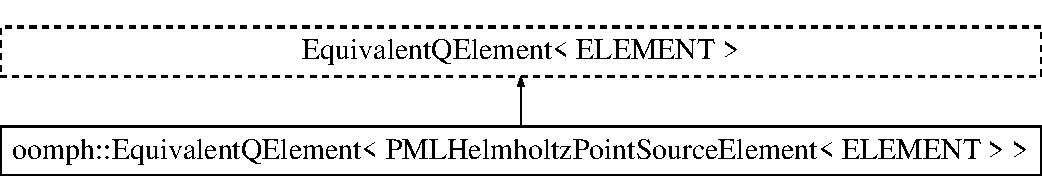
\includegraphics[height=2.000000cm]{classoomph_1_1EquivalentQElement_3_01PMLHelmholtzPointSourceElement_3_01ELEMENT_01_4_01_4}
\end{center}
\end{figure}
\subsection*{Public Member Functions}
\begin{DoxyCompactItemize}
\item 
\hyperlink{classoomph_1_1EquivalentQElement_3_01PMLHelmholtzPointSourceElement_3_01ELEMENT_01_4_01_4_af5fac6bf3394d799567523c3851288f2}{Equivalent\+Q\+Element} ()
\begin{DoxyCompactList}\small\item\em Constructor\+: Call the constructor for the appropriate Element. \end{DoxyCompactList}\end{DoxyCompactItemize}


\subsection{Detailed Description}
\subsubsection*{template$<$class E\+L\+E\+M\+E\+NT$>$\newline
class oomph\+::\+Equivalent\+Q\+Element$<$ P\+M\+L\+Helmholtz\+Point\+Source\+Element$<$ E\+L\+E\+M\+E\+N\+T $>$ $>$}

Policy class defining the elements to be used in the actual P\+ML layers. 

Definition at line 385 of file oscillating\+\_\+sphere.\+cc.



\subsection{Constructor \& Destructor Documentation}
\mbox{\Hypertarget{classoomph_1_1EquivalentQElement_3_01PMLHelmholtzPointSourceElement_3_01ELEMENT_01_4_01_4_af5fac6bf3394d799567523c3851288f2}\label{classoomph_1_1EquivalentQElement_3_01PMLHelmholtzPointSourceElement_3_01ELEMENT_01_4_01_4_af5fac6bf3394d799567523c3851288f2}} 
\index{oomph\+::\+Equivalent\+Q\+Element$<$ P\+M\+L\+Helmholtz\+Point\+Source\+Element$<$ E\+L\+E\+M\+E\+N\+T $>$ $>$@{oomph\+::\+Equivalent\+Q\+Element$<$ P\+M\+L\+Helmholtz\+Point\+Source\+Element$<$ E\+L\+E\+M\+E\+N\+T $>$ $>$}!Equivalent\+Q\+Element@{Equivalent\+Q\+Element}}
\index{Equivalent\+Q\+Element@{Equivalent\+Q\+Element}!oomph\+::\+Equivalent\+Q\+Element$<$ P\+M\+L\+Helmholtz\+Point\+Source\+Element$<$ E\+L\+E\+M\+E\+N\+T $>$ $>$@{oomph\+::\+Equivalent\+Q\+Element$<$ P\+M\+L\+Helmholtz\+Point\+Source\+Element$<$ E\+L\+E\+M\+E\+N\+T $>$ $>$}}
\subsubsection{\texorpdfstring{Equivalent\+Q\+Element()}{EquivalentQElement()}}
{\footnotesize\ttfamily template$<$class E\+L\+E\+M\+E\+NT $>$ \\
oomph\+::\+Equivalent\+Q\+Element$<$ \hyperlink{classoomph_1_1PMLHelmholtzPointSourceElement}{P\+M\+L\+Helmholtz\+Point\+Source\+Element}$<$ E\+L\+E\+M\+E\+NT $>$ $>$\+::Equivalent\+Q\+Element (\begin{DoxyParamCaption}{ }\end{DoxyParamCaption})\hspace{0.3cm}{\ttfamily [inline]}}



Constructor\+: Call the constructor for the appropriate Element. 



Definition at line 393 of file oscillating\+\_\+sphere.\+cc.



The documentation for this class was generated from the following file\+:\begin{DoxyCompactItemize}
\item 
\hyperlink{oscillating__sphere_8cc}{oscillating\+\_\+sphere.\+cc}\end{DoxyCompactItemize}

\hypertarget{classoomph_1_1EquivalentQElement_3_01ProjectablePMLFourierDecomposedHelmholtzElement_3_01PMLHelmea655fba41d5fa485ebddcd1b3c02e7e}{}\section{oomph\+:\+:Equivalent\+Q\+Element$<$ Projectable\+P\+M\+L\+Fourier\+Decomposed\+Helmholtz\+Element$<$ P\+M\+L\+Helmholtz\+Point\+Source\+Element$<$ E\+L\+E\+M\+E\+NT $>$ $>$ $>$ Class Template Reference}
\label{classoomph_1_1EquivalentQElement_3_01ProjectablePMLFourierDecomposedHelmholtzElement_3_01PMLHelmea655fba41d5fa485ebddcd1b3c02e7e}\index{oomph\+::\+Equivalent\+Q\+Element$<$ Projectable\+P\+M\+L\+Fourier\+Decomposed\+Helmholtz\+Element$<$ P\+M\+L\+Helmholtz\+Point\+Source\+Element$<$ E\+L\+E\+M\+E\+N\+T $>$ $>$ $>$@{oomph\+::\+Equivalent\+Q\+Element$<$ Projectable\+P\+M\+L\+Fourier\+Decomposed\+Helmholtz\+Element$<$ P\+M\+L\+Helmholtz\+Point\+Source\+Element$<$ E\+L\+E\+M\+E\+N\+T $>$ $>$ $>$}}
Inheritance diagram for oomph\+:\+:Equivalent\+Q\+Element$<$ Projectable\+P\+M\+L\+Fourier\+Decomposed\+Helmholtz\+Element$<$ P\+M\+L\+Helmholtz\+Point\+Source\+Element$<$ E\+L\+E\+M\+E\+NT $>$ $>$ $>$\+:\begin{figure}[H]
\begin{center}
\leavevmode
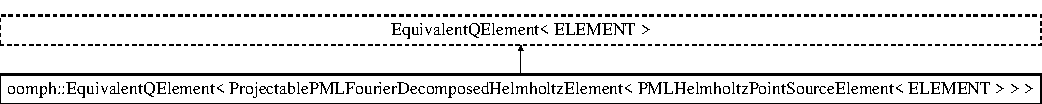
\includegraphics[height=1.398252cm]{classoomph_1_1EquivalentQElement_3_01ProjectablePMLFourierDecomposedHelmholtzElement_3_01PMLHelmea655fba41d5fa485ebddcd1b3c02e7e}
\end{center}
\end{figure}
\subsection*{Public Member Functions}
\begin{DoxyCompactItemize}
\item 
\hyperlink{classoomph_1_1EquivalentQElement_3_01ProjectablePMLFourierDecomposedHelmholtzElement_3_01PMLHelmea655fba41d5fa485ebddcd1b3c02e7e_a05c08c65ab04f51b45a05c8e7aa11389}{Equivalent\+Q\+Element} ()
\begin{DoxyCompactList}\small\item\em Constructor\+: Call the constructor for the appropriate Element. \end{DoxyCompactList}\end{DoxyCompactItemize}


\subsection{Detailed Description}
\subsubsection*{template$<$class E\+L\+E\+M\+E\+NT$>$\newline
class oomph\+::\+Equivalent\+Q\+Element$<$ Projectable\+P\+M\+L\+Fourier\+Decomposed\+Helmholtz\+Element$<$ P\+M\+L\+Helmholtz\+Point\+Source\+Element$<$ E\+L\+E\+M\+E\+N\+T $>$ $>$ $>$}

Policy class defining the elements to be used in the actual P\+ML layers. 

Definition at line 405 of file oscillating\+\_\+sphere.\+cc.



\subsection{Constructor \& Destructor Documentation}
\mbox{\Hypertarget{classoomph_1_1EquivalentQElement_3_01ProjectablePMLFourierDecomposedHelmholtzElement_3_01PMLHelmea655fba41d5fa485ebddcd1b3c02e7e_a05c08c65ab04f51b45a05c8e7aa11389}\label{classoomph_1_1EquivalentQElement_3_01ProjectablePMLFourierDecomposedHelmholtzElement_3_01PMLHelmea655fba41d5fa485ebddcd1b3c02e7e_a05c08c65ab04f51b45a05c8e7aa11389}} 
\index{oomph\+::\+Equivalent\+Q\+Element$<$ Projectable\+P\+M\+L\+Fourier\+Decomposed\+Helmholtz\+Element$<$ P\+M\+L\+Helmholtz\+Point\+Source\+Element$<$ E\+L\+E\+M\+E\+N\+T $>$ $>$ $>$@{oomph\+::\+Equivalent\+Q\+Element$<$ Projectable\+P\+M\+L\+Fourier\+Decomposed\+Helmholtz\+Element$<$ P\+M\+L\+Helmholtz\+Point\+Source\+Element$<$ E\+L\+E\+M\+E\+N\+T $>$ $>$ $>$}!Equivalent\+Q\+Element@{Equivalent\+Q\+Element}}
\index{Equivalent\+Q\+Element@{Equivalent\+Q\+Element}!oomph\+::\+Equivalent\+Q\+Element$<$ Projectable\+P\+M\+L\+Fourier\+Decomposed\+Helmholtz\+Element$<$ P\+M\+L\+Helmholtz\+Point\+Source\+Element$<$ E\+L\+E\+M\+E\+N\+T $>$ $>$ $>$@{oomph\+::\+Equivalent\+Q\+Element$<$ Projectable\+P\+M\+L\+Fourier\+Decomposed\+Helmholtz\+Element$<$ P\+M\+L\+Helmholtz\+Point\+Source\+Element$<$ E\+L\+E\+M\+E\+N\+T $>$ $>$ $>$}}
\subsubsection{\texorpdfstring{Equivalent\+Q\+Element()}{EquivalentQElement()}}
{\footnotesize\ttfamily template$<$class E\+L\+E\+M\+E\+NT $>$ \\
oomph\+::\+Equivalent\+Q\+Element$<$ Projectable\+P\+M\+L\+Fourier\+Decomposed\+Helmholtz\+Element$<$ \hyperlink{classoomph_1_1PMLHelmholtzPointSourceElement}{P\+M\+L\+Helmholtz\+Point\+Source\+Element}$<$ E\+L\+E\+M\+E\+NT $>$ $>$ $>$\+::Equivalent\+Q\+Element (\begin{DoxyParamCaption}{ }\end{DoxyParamCaption})\hspace{0.3cm}{\ttfamily [inline]}}



Constructor\+: Call the constructor for the appropriate Element. 



Definition at line 415 of file oscillating\+\_\+sphere.\+cc.



The documentation for this class was generated from the following file\+:\begin{DoxyCompactItemize}
\item 
\hyperlink{oscillating__sphere_8cc}{oscillating\+\_\+sphere.\+cc}\end{DoxyCompactItemize}

\hypertarget{classoomph_1_1FaceGeometry_3_01FaceGeometry_3_01PMLHelmholtzPointSourceElement_3_01ELEMENT_01_4_01_4_01_4}{}\section{oomph\+:\+:Face\+Geometry$<$ Face\+Geometry$<$ P\+M\+L\+Helmholtz\+Point\+Source\+Element$<$ E\+L\+E\+M\+E\+NT $>$ $>$ $>$ Class Template Reference}
\label{classoomph_1_1FaceGeometry_3_01FaceGeometry_3_01PMLHelmholtzPointSourceElement_3_01ELEMENT_01_4_01_4_01_4}\index{oomph\+::\+Face\+Geometry$<$ Face\+Geometry$<$ P\+M\+L\+Helmholtz\+Point\+Source\+Element$<$ E\+L\+E\+M\+E\+N\+T $>$ $>$ $>$@{oomph\+::\+Face\+Geometry$<$ Face\+Geometry$<$ P\+M\+L\+Helmholtz\+Point\+Source\+Element$<$ E\+L\+E\+M\+E\+N\+T $>$ $>$ $>$}}
Inheritance diagram for oomph\+:\+:Face\+Geometry$<$ Face\+Geometry$<$ P\+M\+L\+Helmholtz\+Point\+Source\+Element$<$ E\+L\+E\+M\+E\+NT $>$ $>$ $>$\+:\begin{figure}[H]
\begin{center}
\leavevmode
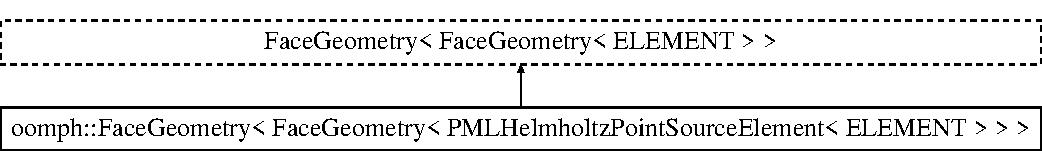
\includegraphics[height=2.000000cm]{classoomph_1_1FaceGeometry_3_01FaceGeometry_3_01PMLHelmholtzPointSourceElement_3_01ELEMENT_01_4_01_4_01_4}
\end{center}
\end{figure}
\subsection*{Public Member Functions}
\begin{DoxyCompactItemize}
\item 
\hyperlink{classoomph_1_1FaceGeometry_3_01FaceGeometry_3_01PMLHelmholtzPointSourceElement_3_01ELEMENT_01_4_01_4_01_4_a5f758bdf1350e4b9a2cea1bcfa26df76}{Face\+Geometry} ()
\end{DoxyCompactItemize}


\subsection{Detailed Description}
\subsubsection*{template$<$class E\+L\+E\+M\+E\+NT$>$\newline
class oomph\+::\+Face\+Geometry$<$ Face\+Geometry$<$ P\+M\+L\+Helmholtz\+Point\+Source\+Element$<$ E\+L\+E\+M\+E\+N\+T $>$ $>$ $>$}

Face geometry of the Face Geometry for element is the same as that for the underlying wrapped element 

Definition at line 372 of file oscillating\+\_\+sphere.\+cc.



\subsection{Constructor \& Destructor Documentation}
\mbox{\Hypertarget{classoomph_1_1FaceGeometry_3_01FaceGeometry_3_01PMLHelmholtzPointSourceElement_3_01ELEMENT_01_4_01_4_01_4_a5f758bdf1350e4b9a2cea1bcfa26df76}\label{classoomph_1_1FaceGeometry_3_01FaceGeometry_3_01PMLHelmholtzPointSourceElement_3_01ELEMENT_01_4_01_4_01_4_a5f758bdf1350e4b9a2cea1bcfa26df76}} 
\index{oomph\+::\+Face\+Geometry$<$ Face\+Geometry$<$ P\+M\+L\+Helmholtz\+Point\+Source\+Element$<$ E\+L\+E\+M\+E\+N\+T $>$ $>$ $>$@{oomph\+::\+Face\+Geometry$<$ Face\+Geometry$<$ P\+M\+L\+Helmholtz\+Point\+Source\+Element$<$ E\+L\+E\+M\+E\+N\+T $>$ $>$ $>$}!Face\+Geometry@{Face\+Geometry}}
\index{Face\+Geometry@{Face\+Geometry}!oomph\+::\+Face\+Geometry$<$ Face\+Geometry$<$ P\+M\+L\+Helmholtz\+Point\+Source\+Element$<$ E\+L\+E\+M\+E\+N\+T $>$ $>$ $>$@{oomph\+::\+Face\+Geometry$<$ Face\+Geometry$<$ P\+M\+L\+Helmholtz\+Point\+Source\+Element$<$ E\+L\+E\+M\+E\+N\+T $>$ $>$ $>$}}
\subsubsection{\texorpdfstring{Face\+Geometry()}{FaceGeometry()}}
{\footnotesize\ttfamily template$<$class E\+L\+E\+M\+E\+NT $>$ \\
oomph\+::\+Face\+Geometry$<$ Face\+Geometry$<$ \hyperlink{classoomph_1_1PMLHelmholtzPointSourceElement}{P\+M\+L\+Helmholtz\+Point\+Source\+Element}$<$ E\+L\+E\+M\+E\+NT $>$ $>$ $>$\+::Face\+Geometry (\begin{DoxyParamCaption}{ }\end{DoxyParamCaption})\hspace{0.3cm}{\ttfamily [inline]}}



Definition at line 376 of file oscillating\+\_\+sphere.\+cc.



The documentation for this class was generated from the following file\+:\begin{DoxyCompactItemize}
\item 
\hyperlink{oscillating__sphere_8cc}{oscillating\+\_\+sphere.\+cc}\end{DoxyCompactItemize}

\hypertarget{classoomph_1_1FaceGeometry_3_01PMLHelmholtzPointSourceElement_3_01ELEMENT_01_4_01_4}{}\section{oomph\+:\+:Face\+Geometry$<$ P\+M\+L\+Helmholtz\+Point\+Source\+Element$<$ E\+L\+E\+M\+E\+NT $>$ $>$ Class Template Reference}
\label{classoomph_1_1FaceGeometry_3_01PMLHelmholtzPointSourceElement_3_01ELEMENT_01_4_01_4}\index{oomph\+::\+Face\+Geometry$<$ P\+M\+L\+Helmholtz\+Point\+Source\+Element$<$ E\+L\+E\+M\+E\+N\+T $>$ $>$@{oomph\+::\+Face\+Geometry$<$ P\+M\+L\+Helmholtz\+Point\+Source\+Element$<$ E\+L\+E\+M\+E\+N\+T $>$ $>$}}
Inheritance diagram for oomph\+:\+:Face\+Geometry$<$ P\+M\+L\+Helmholtz\+Point\+Source\+Element$<$ E\+L\+E\+M\+E\+NT $>$ $>$\+:\begin{figure}[H]
\begin{center}
\leavevmode
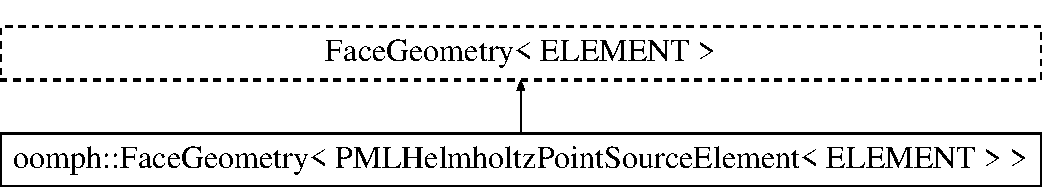
\includegraphics[height=2.000000cm]{classoomph_1_1FaceGeometry_3_01PMLHelmholtzPointSourceElement_3_01ELEMENT_01_4_01_4}
\end{center}
\end{figure}
\subsection*{Public Member Functions}
\begin{DoxyCompactItemize}
\item 
\hyperlink{classoomph_1_1FaceGeometry_3_01PMLHelmholtzPointSourceElement_3_01ELEMENT_01_4_01_4_abf99f385b7c32969fdef43209e14ce79}{Face\+Geometry} ()
\end{DoxyCompactItemize}


\subsection{Detailed Description}
\subsubsection*{template$<$class E\+L\+E\+M\+E\+NT$>$\newline
class oomph\+::\+Face\+Geometry$<$ P\+M\+L\+Helmholtz\+Point\+Source\+Element$<$ E\+L\+E\+M\+E\+N\+T $>$ $>$}

Face geometry for element is the same as that for the underlying wrapped element 

Definition at line 359 of file oscillating\+\_\+sphere.\+cc.



\subsection{Constructor \& Destructor Documentation}
\mbox{\Hypertarget{classoomph_1_1FaceGeometry_3_01PMLHelmholtzPointSourceElement_3_01ELEMENT_01_4_01_4_abf99f385b7c32969fdef43209e14ce79}\label{classoomph_1_1FaceGeometry_3_01PMLHelmholtzPointSourceElement_3_01ELEMENT_01_4_01_4_abf99f385b7c32969fdef43209e14ce79}} 
\index{oomph\+::\+Face\+Geometry$<$ P\+M\+L\+Helmholtz\+Point\+Source\+Element$<$ E\+L\+E\+M\+E\+N\+T $>$ $>$@{oomph\+::\+Face\+Geometry$<$ P\+M\+L\+Helmholtz\+Point\+Source\+Element$<$ E\+L\+E\+M\+E\+N\+T $>$ $>$}!Face\+Geometry@{Face\+Geometry}}
\index{Face\+Geometry@{Face\+Geometry}!oomph\+::\+Face\+Geometry$<$ P\+M\+L\+Helmholtz\+Point\+Source\+Element$<$ E\+L\+E\+M\+E\+N\+T $>$ $>$@{oomph\+::\+Face\+Geometry$<$ P\+M\+L\+Helmholtz\+Point\+Source\+Element$<$ E\+L\+E\+M\+E\+N\+T $>$ $>$}}
\subsubsection{\texorpdfstring{Face\+Geometry()}{FaceGeometry()}}
{\footnotesize\ttfamily template$<$class E\+L\+E\+M\+E\+NT $>$ \\
oomph\+::\+Face\+Geometry$<$ \hyperlink{classoomph_1_1PMLHelmholtzPointSourceElement}{P\+M\+L\+Helmholtz\+Point\+Source\+Element}$<$ E\+L\+E\+M\+E\+NT $>$ $>$\+::Face\+Geometry (\begin{DoxyParamCaption}{ }\end{DoxyParamCaption})\hspace{0.3cm}{\ttfamily [inline]}}



Definition at line 363 of file oscillating\+\_\+sphere.\+cc.



The documentation for this class was generated from the following file\+:\begin{DoxyCompactItemize}
\item 
\hyperlink{oscillating__sphere_8cc}{oscillating\+\_\+sphere.\+cc}\end{DoxyCompactItemize}

\hypertarget{classPMLFourierDecomposedHelmholtzProblem}{}\section{P\+M\+L\+Fourier\+Decomposed\+Helmholtz\+Problem$<$ E\+L\+E\+M\+E\+NT $>$ Class Template Reference}
\label{classPMLFourierDecomposedHelmholtzProblem}\index{P\+M\+L\+Fourier\+Decomposed\+Helmholtz\+Problem$<$ E\+L\+E\+M\+E\+N\+T $>$@{P\+M\+L\+Fourier\+Decomposed\+Helmholtz\+Problem$<$ E\+L\+E\+M\+E\+N\+T $>$}}


Problem class.  


Inheritance diagram for P\+M\+L\+Fourier\+Decomposed\+Helmholtz\+Problem$<$ E\+L\+E\+M\+E\+NT $>$\+:\begin{figure}[H]
\begin{center}
\leavevmode
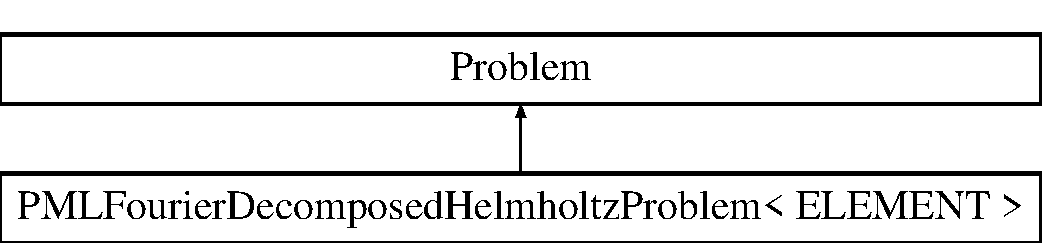
\includegraphics[height=2.000000cm]{classPMLFourierDecomposedHelmholtzProblem}
\end{center}
\end{figure}
\subsection*{Public Member Functions}
\begin{DoxyCompactItemize}
\item 
\hyperlink{classPMLFourierDecomposedHelmholtzProblem_a5764db8312a28a3e1eaac2cc61813f83}{P\+M\+L\+Fourier\+Decomposed\+Helmholtz\+Problem} ()
\begin{DoxyCompactList}\small\item\em Constructor. \end{DoxyCompactList}\item 
\hyperlink{classPMLFourierDecomposedHelmholtzProblem_abc35779657bcdd622d09464c225b079a}{$\sim$\+P\+M\+L\+Fourier\+Decomposed\+Helmholtz\+Problem} ()
\begin{DoxyCompactList}\small\item\em Destructor (empty) \end{DoxyCompactList}\item 
void \hyperlink{classPMLFourierDecomposedHelmholtzProblem_af87810cbe164981cc14ee779793a69fb}{actions\+\_\+before\+\_\+newton\+\_\+solve} ()
\begin{DoxyCompactList}\small\item\em Update the problem specs before solve (empty) \end{DoxyCompactList}\item 
void \hyperlink{classPMLFourierDecomposedHelmholtzProblem_a013d95d489b85e326a71bb744af4a40f}{actions\+\_\+after\+\_\+newton\+\_\+solve} ()
\begin{DoxyCompactList}\small\item\em Update the problem after solve (empty) \end{DoxyCompactList}\item 
void \hyperlink{classPMLFourierDecomposedHelmholtzProblem_afcdfaf86efc75fbea14f6ade9eeb7f9c}{doc\+\_\+solution} (Doc\+Info \&doc\+\_\+info)
\begin{DoxyCompactList}\small\item\em Doc the solution. Doc\+Info object stores flags/labels for where the output gets written to. \end{DoxyCompactList}\item 
void \hyperlink{classPMLFourierDecomposedHelmholtzProblem_ae562dddf5c60793371b594bff5047f91}{create\+\_\+pml\+\_\+meshes} ()
\begin{DoxyCompactList}\small\item\em Create P\+ML meshes. \end{DoxyCompactList}\item 
void \hyperlink{classPMLFourierDecomposedHelmholtzProblem_a83e0aa333ec3b25f1afccc3bc0a529ad}{create\+\_\+power\+\_\+monitor\+\_\+mesh} ()
\begin{DoxyCompactList}\small\item\em Create mesh of face elements that monitor the radiated power. \end{DoxyCompactList}\item 
void \hyperlink{classPMLFourierDecomposedHelmholtzProblem_ae4b1cacec10553bdb6781b65ed73abce}{actions\+\_\+before\+\_\+adapt} ()
\begin{DoxyCompactList}\small\item\em Actions before adapt\+: Wipe the mesh of prescribed flux elements. \end{DoxyCompactList}\item 
void \hyperlink{classPMLFourierDecomposedHelmholtzProblem_ad19bce2b8cb30bdeffd656fdc4014c0c}{actions\+\_\+after\+\_\+adapt} ()
\begin{DoxyCompactList}\small\item\em Actions after adapt\+: Rebuild the mesh of prescribed flux elements. \end{DoxyCompactList}\item 
void \hyperlink{classPMLFourierDecomposedHelmholtzProblem_aca49343d9672607fdc3ab5f6ed4e9d24}{complete\+\_\+problem\+\_\+setup} ()
\end{DoxyCompactItemize}
\subsection*{Private Member Functions}
\begin{DoxyCompactItemize}
\item 
void \hyperlink{classPMLFourierDecomposedHelmholtzProblem_afd6e3401bdbd1d3deb3271553fbe1d3a}{create\+\_\+flux\+\_\+elements\+\_\+on\+\_\+inner\+\_\+boundary} ()
\begin{DoxyCompactList}\small\item\em Create flux elements on inner boundary. \end{DoxyCompactList}\item 
void \hyperlink{classPMLFourierDecomposedHelmholtzProblem_a4a9b767ba4beb7ab5db9c98fc46c49b2}{delete\+\_\+face\+\_\+elements} (Mesh $\ast$const \&boundary\+\_\+mesh\+\_\+pt)
\begin{DoxyCompactList}\small\item\em Delete boundary face elements and wipe the surface mesh. \end{DoxyCompactList}\item 
void \hyperlink{classPMLFourierDecomposedHelmholtzProblem_ad7680c25a32087cb6da96d4bcedf1b23}{apply\+\_\+zero\+\_\+dirichlet\+\_\+boundary\+\_\+conditions} ()
\item 
void \hyperlink{classPMLFourierDecomposedHelmholtzProblem_a7d416452acc602776de2072a7c0e1249}{setup\+\_\+point\+\_\+source} ()
\begin{DoxyCompactList}\small\item\em Set point source. \end{DoxyCompactList}\end{DoxyCompactItemize}
\subsection*{Private Attributes}
\begin{DoxyCompactItemize}
\item 
Mesh $\ast$ \hyperlink{classPMLFourierDecomposedHelmholtzProblem_a9ffebfa69944e405eb28a4b2bd03336e}{Power\+\_\+monitor\+\_\+mesh\+\_\+pt}
\begin{DoxyCompactList}\small\item\em Pointer to mesh that stores the power monitor elements. \end{DoxyCompactList}\item 
Refineable\+Triangle\+Mesh$<$ E\+L\+E\+M\+E\+NT $>$ $\ast$ \hyperlink{classPMLFourierDecomposedHelmholtzProblem_ad20477e869fb9ce66891389c0d501449}{Bulk\+\_\+mesh\+\_\+pt}
\begin{DoxyCompactList}\small\item\em Pointer to the refineable \char`\"{}bulk\char`\"{} mesh. \end{DoxyCompactList}\item 
Mesh\+As\+Geom\+Object $\ast$ \hyperlink{classPMLFourierDecomposedHelmholtzProblem_a32f6694310ffd9c0962a7ee8c114dbf5}{Mesh\+\_\+as\+\_\+geom\+\_\+obj\+\_\+pt}
\begin{DoxyCompactList}\small\item\em Mesh as geometric object representation of bulk mesh. \end{DoxyCompactList}\item 
Triangle\+Mesh$<$ E\+L\+E\+M\+E\+NT $>$ $\ast$ \hyperlink{classPMLFourierDecomposedHelmholtzProblem_a583fb8d30b3a225fe77f684532efd66f}{Bulk\+\_\+mesh\+\_\+pt}
\begin{DoxyCompactList}\small\item\em Pointer to the \char`\"{}bulk\char`\"{} mesh. \end{DoxyCompactList}\item 
Mesh $\ast$ \hyperlink{classPMLFourierDecomposedHelmholtzProblem_a7d3c418942daf7ba2363b8a91172512e}{Helmholtz\+\_\+inner\+\_\+boundary\+\_\+mesh\+\_\+pt}
\begin{DoxyCompactList}\small\item\em Mesh of Face\+Elements that apply the flux bc on the inner boundary. \end{DoxyCompactList}\item 
Mesh $\ast$ \hyperlink{classPMLFourierDecomposedHelmholtzProblem_a2bde26fe496f63d29e48e9b5dffc8757}{P\+M\+L\+\_\+right\+\_\+mesh\+\_\+pt}
\begin{DoxyCompactList}\small\item\em Pointer to the right P\+ML mesh. \end{DoxyCompactList}\item 
Mesh $\ast$ \hyperlink{classPMLFourierDecomposedHelmholtzProblem_a4fe4cd439faae2086ab1ed786cbc610a}{P\+M\+L\+\_\+top\+\_\+mesh\+\_\+pt}
\begin{DoxyCompactList}\small\item\em Pointer to the top P\+ML mesh. \end{DoxyCompactList}\item 
Mesh $\ast$ \hyperlink{classPMLFourierDecomposedHelmholtzProblem_ad7611d07d182b33a5e2f848bc4ff5572}{P\+M\+L\+\_\+bottom\+\_\+mesh\+\_\+pt}
\begin{DoxyCompactList}\small\item\em Pointer to the bottom P\+ML mesh. \end{DoxyCompactList}\item 
Mesh $\ast$ \hyperlink{classPMLFourierDecomposedHelmholtzProblem_af0787c8610bbae59be3d061e57072c11}{P\+M\+L\+\_\+top\+\_\+right\+\_\+mesh\+\_\+pt}
\begin{DoxyCompactList}\small\item\em Pointer to the top right corner P\+ML mesh. \end{DoxyCompactList}\item 
Mesh $\ast$ \hyperlink{classPMLFourierDecomposedHelmholtzProblem_a8c3d30400cb9e4a709e1f8f8ee66785a}{P\+M\+L\+\_\+bottom\+\_\+right\+\_\+mesh\+\_\+pt}
\begin{DoxyCompactList}\small\item\em Pointer to the bottom right corner P\+ML mesh. \end{DoxyCompactList}\item 
ofstream \hyperlink{classPMLFourierDecomposedHelmholtzProblem_a9810d1dd58cec1f8b1cfc54ea37a7efd}{Trace\+\_\+file}
\begin{DoxyCompactList}\small\item\em Trace file. \end{DoxyCompactList}\end{DoxyCompactItemize}


\subsection{Detailed Description}
\subsubsection*{template$<$class E\+L\+E\+M\+E\+NT$>$\newline
class P\+M\+L\+Fourier\+Decomposed\+Helmholtz\+Problem$<$ E\+L\+E\+M\+E\+N\+T $>$}

Problem class. 

Definition at line 433 of file oscillating\+\_\+sphere.\+cc.



\subsection{Constructor \& Destructor Documentation}
\mbox{\Hypertarget{classPMLFourierDecomposedHelmholtzProblem_a5764db8312a28a3e1eaac2cc61813f83}\label{classPMLFourierDecomposedHelmholtzProblem_a5764db8312a28a3e1eaac2cc61813f83}} 
\index{P\+M\+L\+Fourier\+Decomposed\+Helmholtz\+Problem@{P\+M\+L\+Fourier\+Decomposed\+Helmholtz\+Problem}!P\+M\+L\+Fourier\+Decomposed\+Helmholtz\+Problem@{P\+M\+L\+Fourier\+Decomposed\+Helmholtz\+Problem}}
\index{P\+M\+L\+Fourier\+Decomposed\+Helmholtz\+Problem@{P\+M\+L\+Fourier\+Decomposed\+Helmholtz\+Problem}!P\+M\+L\+Fourier\+Decomposed\+Helmholtz\+Problem@{P\+M\+L\+Fourier\+Decomposed\+Helmholtz\+Problem}}
\subsubsection{\texorpdfstring{P\+M\+L\+Fourier\+Decomposed\+Helmholtz\+Problem()}{PMLFourierDecomposedHelmholtzProblem()}}
{\footnotesize\ttfamily template$<$class E\+L\+E\+M\+E\+NT $>$ \\
\hyperlink{classPMLFourierDecomposedHelmholtzProblem}{P\+M\+L\+Fourier\+Decomposed\+Helmholtz\+Problem}$<$ E\+L\+E\+M\+E\+NT $>$\+::\hyperlink{classPMLFourierDecomposedHelmholtzProblem}{P\+M\+L\+Fourier\+Decomposed\+Helmholtz\+Problem} (\begin{DoxyParamCaption}{ }\end{DoxyParamCaption})}



Constructor. 

Constructor for Pml Fourier-\/decomposed Helmholtz problem. Setup \char`\"{}bulk\char`\"{} mesh 

Definition at line 794 of file oscillating\+\_\+sphere.\+cc.



References Problem\+Parameters\+::\+Directory, P\+M\+L\+Fourier\+Decomposed\+Helmholtz\+Problem$<$ E\+L\+E\+M\+E\+N\+T $>$\+::doc\+\_\+solution(), Problem\+Parameters\+::\+Element\+\_\+area, and Problem\+Parameters\+::\+K\+\_\+squared.



Referenced by P\+M\+L\+Fourier\+Decomposed\+Helmholtz\+Problem$<$ E\+L\+E\+M\+E\+N\+T $>$\+::apply\+\_\+zero\+\_\+dirichlet\+\_\+boundary\+\_\+conditions().

\mbox{\Hypertarget{classPMLFourierDecomposedHelmholtzProblem_abc35779657bcdd622d09464c225b079a}\label{classPMLFourierDecomposedHelmholtzProblem_abc35779657bcdd622d09464c225b079a}} 
\index{P\+M\+L\+Fourier\+Decomposed\+Helmholtz\+Problem@{P\+M\+L\+Fourier\+Decomposed\+Helmholtz\+Problem}!````~P\+M\+L\+Fourier\+Decomposed\+Helmholtz\+Problem@{$\sim$\+P\+M\+L\+Fourier\+Decomposed\+Helmholtz\+Problem}}
\index{````~P\+M\+L\+Fourier\+Decomposed\+Helmholtz\+Problem@{$\sim$\+P\+M\+L\+Fourier\+Decomposed\+Helmholtz\+Problem}!P\+M\+L\+Fourier\+Decomposed\+Helmholtz\+Problem@{P\+M\+L\+Fourier\+Decomposed\+Helmholtz\+Problem}}
\subsubsection{\texorpdfstring{$\sim$\+P\+M\+L\+Fourier\+Decomposed\+Helmholtz\+Problem()}{~PMLFourierDecomposedHelmholtzProblem()}}
{\footnotesize\ttfamily template$<$class E\+L\+E\+M\+E\+NT $>$ \\
\hyperlink{classPMLFourierDecomposedHelmholtzProblem}{P\+M\+L\+Fourier\+Decomposed\+Helmholtz\+Problem}$<$ E\+L\+E\+M\+E\+NT $>$\+::$\sim$\hyperlink{classPMLFourierDecomposedHelmholtzProblem}{P\+M\+L\+Fourier\+Decomposed\+Helmholtz\+Problem} (\begin{DoxyParamCaption}{ }\end{DoxyParamCaption})\hspace{0.3cm}{\ttfamily [inline]}}



Destructor (empty) 



Definition at line 442 of file oscillating\+\_\+sphere.\+cc.



\subsection{Member Function Documentation}
\mbox{\Hypertarget{classPMLFourierDecomposedHelmholtzProblem_ad19bce2b8cb30bdeffd656fdc4014c0c}\label{classPMLFourierDecomposedHelmholtzProblem_ad19bce2b8cb30bdeffd656fdc4014c0c}} 
\index{P\+M\+L\+Fourier\+Decomposed\+Helmholtz\+Problem@{P\+M\+L\+Fourier\+Decomposed\+Helmholtz\+Problem}!actions\+\_\+after\+\_\+adapt@{actions\+\_\+after\+\_\+adapt}}
\index{actions\+\_\+after\+\_\+adapt@{actions\+\_\+after\+\_\+adapt}!P\+M\+L\+Fourier\+Decomposed\+Helmholtz\+Problem@{P\+M\+L\+Fourier\+Decomposed\+Helmholtz\+Problem}}
\subsubsection{\texorpdfstring{actions\+\_\+after\+\_\+adapt()}{actions\_after\_adapt()}}
{\footnotesize\ttfamily template$<$class E\+L\+E\+M\+E\+NT $>$ \\
void \hyperlink{classPMLFourierDecomposedHelmholtzProblem}{P\+M\+L\+Fourier\+Decomposed\+Helmholtz\+Problem}$<$ E\+L\+E\+M\+E\+NT $>$\+::actions\+\_\+after\+\_\+adapt (\begin{DoxyParamCaption}{ }\end{DoxyParamCaption})}



Actions after adapt\+: Rebuild the mesh of prescribed flux elements. 

Actions after adapt\+: Rebuild the face element meshes. 

Definition at line 623 of file oscillating\+\_\+sphere.\+cc.



References P\+M\+L\+Fourier\+Decomposed\+Helmholtz\+Problem$<$ E\+L\+E\+M\+E\+N\+T $>$\+::complete\+\_\+problem\+\_\+setup().



Referenced by P\+M\+L\+Fourier\+Decomposed\+Helmholtz\+Problem$<$ E\+L\+E\+M\+E\+N\+T $>$\+::actions\+\_\+before\+\_\+adapt().

\mbox{\Hypertarget{classPMLFourierDecomposedHelmholtzProblem_a013d95d489b85e326a71bb744af4a40f}\label{classPMLFourierDecomposedHelmholtzProblem_a013d95d489b85e326a71bb744af4a40f}} 
\index{P\+M\+L\+Fourier\+Decomposed\+Helmholtz\+Problem@{P\+M\+L\+Fourier\+Decomposed\+Helmholtz\+Problem}!actions\+\_\+after\+\_\+newton\+\_\+solve@{actions\+\_\+after\+\_\+newton\+\_\+solve}}
\index{actions\+\_\+after\+\_\+newton\+\_\+solve@{actions\+\_\+after\+\_\+newton\+\_\+solve}!P\+M\+L\+Fourier\+Decomposed\+Helmholtz\+Problem@{P\+M\+L\+Fourier\+Decomposed\+Helmholtz\+Problem}}
\subsubsection{\texorpdfstring{actions\+\_\+after\+\_\+newton\+\_\+solve()}{actions\_after\_newton\_solve()}}
{\footnotesize\ttfamily template$<$class E\+L\+E\+M\+E\+NT $>$ \\
void \hyperlink{classPMLFourierDecomposedHelmholtzProblem}{P\+M\+L\+Fourier\+Decomposed\+Helmholtz\+Problem}$<$ E\+L\+E\+M\+E\+NT $>$\+::actions\+\_\+after\+\_\+newton\+\_\+solve (\begin{DoxyParamCaption}{ }\end{DoxyParamCaption})\hspace{0.3cm}{\ttfamily [inline]}}



Update the problem after solve (empty) 



Definition at line 448 of file oscillating\+\_\+sphere.\+cc.

\mbox{\Hypertarget{classPMLFourierDecomposedHelmholtzProblem_ae4b1cacec10553bdb6781b65ed73abce}\label{classPMLFourierDecomposedHelmholtzProblem_ae4b1cacec10553bdb6781b65ed73abce}} 
\index{P\+M\+L\+Fourier\+Decomposed\+Helmholtz\+Problem@{P\+M\+L\+Fourier\+Decomposed\+Helmholtz\+Problem}!actions\+\_\+before\+\_\+adapt@{actions\+\_\+before\+\_\+adapt}}
\index{actions\+\_\+before\+\_\+adapt@{actions\+\_\+before\+\_\+adapt}!P\+M\+L\+Fourier\+Decomposed\+Helmholtz\+Problem@{P\+M\+L\+Fourier\+Decomposed\+Helmholtz\+Problem}}
\subsubsection{\texorpdfstring{actions\+\_\+before\+\_\+adapt()}{actions\_before\_adapt()}}
{\footnotesize\ttfamily template$<$class E\+L\+E\+M\+E\+NT $>$ \\
void \hyperlink{classPMLFourierDecomposedHelmholtzProblem}{P\+M\+L\+Fourier\+Decomposed\+Helmholtz\+Problem}$<$ E\+L\+E\+M\+E\+NT $>$\+::actions\+\_\+before\+\_\+adapt (\begin{DoxyParamCaption}{ }\end{DoxyParamCaption})}



Actions before adapt\+: Wipe the mesh of prescribed flux elements. 

Actions before adapt\+: Wipe the mesh of face elements. 

Definition at line 585 of file oscillating\+\_\+sphere.\+cc.



References P\+M\+L\+Fourier\+Decomposed\+Helmholtz\+Problem$<$ E\+L\+E\+M\+E\+N\+T $>$\+::actions\+\_\+after\+\_\+adapt().



Referenced by P\+M\+L\+Fourier\+Decomposed\+Helmholtz\+Problem$<$ E\+L\+E\+M\+E\+N\+T $>$\+::create\+\_\+power\+\_\+monitor\+\_\+mesh().

\mbox{\Hypertarget{classPMLFourierDecomposedHelmholtzProblem_af87810cbe164981cc14ee779793a69fb}\label{classPMLFourierDecomposedHelmholtzProblem_af87810cbe164981cc14ee779793a69fb}} 
\index{P\+M\+L\+Fourier\+Decomposed\+Helmholtz\+Problem@{P\+M\+L\+Fourier\+Decomposed\+Helmholtz\+Problem}!actions\+\_\+before\+\_\+newton\+\_\+solve@{actions\+\_\+before\+\_\+newton\+\_\+solve}}
\index{actions\+\_\+before\+\_\+newton\+\_\+solve@{actions\+\_\+before\+\_\+newton\+\_\+solve}!P\+M\+L\+Fourier\+Decomposed\+Helmholtz\+Problem@{P\+M\+L\+Fourier\+Decomposed\+Helmholtz\+Problem}}
\subsubsection{\texorpdfstring{actions\+\_\+before\+\_\+newton\+\_\+solve()}{actions\_before\_newton\_solve()}}
{\footnotesize\ttfamily template$<$class E\+L\+E\+M\+E\+NT $>$ \\
void \hyperlink{classPMLFourierDecomposedHelmholtzProblem}{P\+M\+L\+Fourier\+Decomposed\+Helmholtz\+Problem}$<$ E\+L\+E\+M\+E\+NT $>$\+::actions\+\_\+before\+\_\+newton\+\_\+solve (\begin{DoxyParamCaption}{ }\end{DoxyParamCaption})\hspace{0.3cm}{\ttfamily [inline]}}



Update the problem specs before solve (empty) 



Definition at line 445 of file oscillating\+\_\+sphere.\+cc.

\mbox{\Hypertarget{classPMLFourierDecomposedHelmholtzProblem_ad7680c25a32087cb6da96d4bcedf1b23}\label{classPMLFourierDecomposedHelmholtzProblem_ad7680c25a32087cb6da96d4bcedf1b23}} 
\index{P\+M\+L\+Fourier\+Decomposed\+Helmholtz\+Problem@{P\+M\+L\+Fourier\+Decomposed\+Helmholtz\+Problem}!apply\+\_\+zero\+\_\+dirichlet\+\_\+boundary\+\_\+conditions@{apply\+\_\+zero\+\_\+dirichlet\+\_\+boundary\+\_\+conditions}}
\index{apply\+\_\+zero\+\_\+dirichlet\+\_\+boundary\+\_\+conditions@{apply\+\_\+zero\+\_\+dirichlet\+\_\+boundary\+\_\+conditions}!P\+M\+L\+Fourier\+Decomposed\+Helmholtz\+Problem@{P\+M\+L\+Fourier\+Decomposed\+Helmholtz\+Problem}}
\subsubsection{\texorpdfstring{apply\+\_\+zero\+\_\+dirichlet\+\_\+boundary\+\_\+conditions()}{apply\_zero\_dirichlet\_boundary\_conditions()}}
{\footnotesize\ttfamily template$<$class E\+L\+E\+M\+E\+NT $>$ \\
void \hyperlink{classPMLFourierDecomposedHelmholtzProblem}{P\+M\+L\+Fourier\+Decomposed\+Helmholtz\+Problem}$<$ E\+L\+E\+M\+E\+NT $>$\+::apply\+\_\+zero\+\_\+dirichlet\+\_\+boundary\+\_\+conditions (\begin{DoxyParamCaption}{ }\end{DoxyParamCaption})\hspace{0.3cm}{\ttfamily [private]}}



Definition at line 736 of file oscillating\+\_\+sphere.\+cc.



References P\+M\+L\+Fourier\+Decomposed\+Helmholtz\+Problem$<$ E\+L\+E\+M\+E\+N\+T $>$\+::\+P\+M\+L\+Fourier\+Decomposed\+Helmholtz\+Problem().



Referenced by P\+M\+L\+Fourier\+Decomposed\+Helmholtz\+Problem$<$ E\+L\+E\+M\+E\+N\+T $>$\+::setup\+\_\+point\+\_\+source().

\mbox{\Hypertarget{classPMLFourierDecomposedHelmholtzProblem_aca49343d9672607fdc3ab5f6ed4e9d24}\label{classPMLFourierDecomposedHelmholtzProblem_aca49343d9672607fdc3ab5f6ed4e9d24}} 
\index{P\+M\+L\+Fourier\+Decomposed\+Helmholtz\+Problem@{P\+M\+L\+Fourier\+Decomposed\+Helmholtz\+Problem}!complete\+\_\+problem\+\_\+setup@{complete\+\_\+problem\+\_\+setup}}
\index{complete\+\_\+problem\+\_\+setup@{complete\+\_\+problem\+\_\+setup}!P\+M\+L\+Fourier\+Decomposed\+Helmholtz\+Problem@{P\+M\+L\+Fourier\+Decomposed\+Helmholtz\+Problem}}
\subsubsection{\texorpdfstring{complete\+\_\+problem\+\_\+setup()}{complete\_problem\_setup()}}
{\footnotesize\ttfamily template$<$class E\+L\+E\+M\+E\+NT $>$ \\
void \hyperlink{classPMLFourierDecomposedHelmholtzProblem}{P\+M\+L\+Fourier\+Decomposed\+Helmholtz\+Problem}$<$ E\+L\+E\+M\+E\+NT $>$\+::complete\+\_\+problem\+\_\+setup (\begin{DoxyParamCaption}{ }\end{DoxyParamCaption})}



Definition at line 653 of file oscillating\+\_\+sphere.\+cc.



References Problem\+Parameters\+::\+K\+\_\+squared, Problem\+Parameters\+::\+N\+\_\+fourier, and P\+M\+L\+Fourier\+Decomposed\+Helmholtz\+Problem$<$ E\+L\+E\+M\+E\+N\+T $>$\+::setup\+\_\+point\+\_\+source().



Referenced by P\+M\+L\+Fourier\+Decomposed\+Helmholtz\+Problem$<$ E\+L\+E\+M\+E\+N\+T $>$\+::actions\+\_\+after\+\_\+adapt().

\mbox{\Hypertarget{classPMLFourierDecomposedHelmholtzProblem_afd6e3401bdbd1d3deb3271553fbe1d3a}\label{classPMLFourierDecomposedHelmholtzProblem_afd6e3401bdbd1d3deb3271553fbe1d3a}} 
\index{P\+M\+L\+Fourier\+Decomposed\+Helmholtz\+Problem@{P\+M\+L\+Fourier\+Decomposed\+Helmholtz\+Problem}!create\+\_\+flux\+\_\+elements\+\_\+on\+\_\+inner\+\_\+boundary@{create\+\_\+flux\+\_\+elements\+\_\+on\+\_\+inner\+\_\+boundary}}
\index{create\+\_\+flux\+\_\+elements\+\_\+on\+\_\+inner\+\_\+boundary@{create\+\_\+flux\+\_\+elements\+\_\+on\+\_\+inner\+\_\+boundary}!P\+M\+L\+Fourier\+Decomposed\+Helmholtz\+Problem@{P\+M\+L\+Fourier\+Decomposed\+Helmholtz\+Problem}}
\subsubsection{\texorpdfstring{create\+\_\+flux\+\_\+elements\+\_\+on\+\_\+inner\+\_\+boundary()}{create\_flux\_elements\_on\_inner\_boundary()}}
{\footnotesize\ttfamily template$<$class E\+L\+E\+M\+E\+NT $>$ \\
void \hyperlink{classPMLFourierDecomposedHelmholtzProblem}{P\+M\+L\+Fourier\+Decomposed\+Helmholtz\+Problem}$<$ E\+L\+E\+M\+E\+NT $>$\+::create\+\_\+flux\+\_\+elements\+\_\+on\+\_\+inner\+\_\+boundary (\begin{DoxyParamCaption}{ }\end{DoxyParamCaption})\hspace{0.3cm}{\ttfamily [private]}}



Create flux elements on inner boundary. 



Definition at line 1076 of file oscillating\+\_\+sphere.\+cc.



References Problem\+Parameters\+::exact\+\_\+minus\+\_\+dudr().



Referenced by P\+M\+L\+Fourier\+Decomposed\+Helmholtz\+Problem$<$ E\+L\+E\+M\+E\+N\+T $>$\+::doc\+\_\+solution().

\mbox{\Hypertarget{classPMLFourierDecomposedHelmholtzProblem_ae562dddf5c60793371b594bff5047f91}\label{classPMLFourierDecomposedHelmholtzProblem_ae562dddf5c60793371b594bff5047f91}} 
\index{P\+M\+L\+Fourier\+Decomposed\+Helmholtz\+Problem@{P\+M\+L\+Fourier\+Decomposed\+Helmholtz\+Problem}!create\+\_\+pml\+\_\+meshes@{create\+\_\+pml\+\_\+meshes}}
\index{create\+\_\+pml\+\_\+meshes@{create\+\_\+pml\+\_\+meshes}!P\+M\+L\+Fourier\+Decomposed\+Helmholtz\+Problem@{P\+M\+L\+Fourier\+Decomposed\+Helmholtz\+Problem}}
\subsubsection{\texorpdfstring{create\+\_\+pml\+\_\+meshes()}{create\_pml\_meshes()}}
{\footnotesize\ttfamily template$<$class E\+L\+E\+M\+E\+NT $>$ \\
void \hyperlink{classPMLFourierDecomposedHelmholtzProblem}{P\+M\+L\+Fourier\+Decomposed\+Helmholtz\+Problem}$<$ E\+L\+E\+M\+E\+NT $>$\+::create\+\_\+pml\+\_\+meshes (\begin{DoxyParamCaption}{ }\end{DoxyParamCaption})}



Create P\+ML meshes. 

Create P\+ML meshes and add them to the problem\textquotesingle{}s sub-\/meshes. 

Definition at line 1114 of file oscillating\+\_\+sphere.\+cc.



References Problem\+Parameters\+::\+Nel\+\_\+pml, and Problem\+Parameters\+::\+P\+M\+L\+\_\+thickness.

\mbox{\Hypertarget{classPMLFourierDecomposedHelmholtzProblem_a83e0aa333ec3b25f1afccc3bc0a529ad}\label{classPMLFourierDecomposedHelmholtzProblem_a83e0aa333ec3b25f1afccc3bc0a529ad}} 
\index{P\+M\+L\+Fourier\+Decomposed\+Helmholtz\+Problem@{P\+M\+L\+Fourier\+Decomposed\+Helmholtz\+Problem}!create\+\_\+power\+\_\+monitor\+\_\+mesh@{create\+\_\+power\+\_\+monitor\+\_\+mesh}}
\index{create\+\_\+power\+\_\+monitor\+\_\+mesh@{create\+\_\+power\+\_\+monitor\+\_\+mesh}!P\+M\+L\+Fourier\+Decomposed\+Helmholtz\+Problem@{P\+M\+L\+Fourier\+Decomposed\+Helmholtz\+Problem}}
\subsubsection{\texorpdfstring{create\+\_\+power\+\_\+monitor\+\_\+mesh()}{create\_power\_monitor\_mesh()}}
{\footnotesize\ttfamily template$<$class E\+L\+E\+M\+E\+NT $>$ \\
void \hyperlink{classPMLFourierDecomposedHelmholtzProblem}{P\+M\+L\+Fourier\+Decomposed\+Helmholtz\+Problem}$<$ E\+L\+E\+M\+E\+NT $>$\+::create\+\_\+power\+\_\+monitor\+\_\+mesh (\begin{DoxyParamCaption}{ }\end{DoxyParamCaption})}



Create mesh of face elements that monitor the radiated power. 

Create BC elements on outer boundary. 

Definition at line 548 of file oscillating\+\_\+sphere.\+cc.



References P\+M\+L\+Fourier\+Decomposed\+Helmholtz\+Problem$<$ E\+L\+E\+M\+E\+N\+T $>$\+::actions\+\_\+before\+\_\+adapt().

\mbox{\Hypertarget{classPMLFourierDecomposedHelmholtzProblem_a4a9b767ba4beb7ab5db9c98fc46c49b2}\label{classPMLFourierDecomposedHelmholtzProblem_a4a9b767ba4beb7ab5db9c98fc46c49b2}} 
\index{P\+M\+L\+Fourier\+Decomposed\+Helmholtz\+Problem@{P\+M\+L\+Fourier\+Decomposed\+Helmholtz\+Problem}!delete\+\_\+face\+\_\+elements@{delete\+\_\+face\+\_\+elements}}
\index{delete\+\_\+face\+\_\+elements@{delete\+\_\+face\+\_\+elements}!P\+M\+L\+Fourier\+Decomposed\+Helmholtz\+Problem@{P\+M\+L\+Fourier\+Decomposed\+Helmholtz\+Problem}}
\subsubsection{\texorpdfstring{delete\+\_\+face\+\_\+elements()}{delete\_face\_elements()}}
{\footnotesize\ttfamily template$<$class E\+L\+E\+M\+E\+NT $>$ \\
void \hyperlink{classPMLFourierDecomposedHelmholtzProblem}{P\+M\+L\+Fourier\+Decomposed\+Helmholtz\+Problem}$<$ E\+L\+E\+M\+E\+NT $>$\+::delete\+\_\+face\+\_\+elements (\begin{DoxyParamCaption}\item[{Mesh $\ast$const \&}]{boundary\+\_\+mesh\+\_\+pt }\end{DoxyParamCaption})\hspace{0.3cm}{\ttfamily [inline]}, {\ttfamily [private]}}



Delete boundary face elements and wipe the surface mesh. 



Definition at line 480 of file oscillating\+\_\+sphere.\+cc.

\mbox{\Hypertarget{classPMLFourierDecomposedHelmholtzProblem_afcdfaf86efc75fbea14f6ade9eeb7f9c}\label{classPMLFourierDecomposedHelmholtzProblem_afcdfaf86efc75fbea14f6ade9eeb7f9c}} 
\index{P\+M\+L\+Fourier\+Decomposed\+Helmholtz\+Problem@{P\+M\+L\+Fourier\+Decomposed\+Helmholtz\+Problem}!doc\+\_\+solution@{doc\+\_\+solution}}
\index{doc\+\_\+solution@{doc\+\_\+solution}!P\+M\+L\+Fourier\+Decomposed\+Helmholtz\+Problem@{P\+M\+L\+Fourier\+Decomposed\+Helmholtz\+Problem}}
\subsubsection{\texorpdfstring{doc\+\_\+solution()}{doc\_solution()}}
{\footnotesize\ttfamily template$<$class E\+L\+E\+M\+E\+NT $>$ \\
void \hyperlink{classPMLFourierDecomposedHelmholtzProblem}{P\+M\+L\+Fourier\+Decomposed\+Helmholtz\+Problem}$<$ E\+L\+E\+M\+E\+NT $>$\+::doc\+\_\+solution (\begin{DoxyParamCaption}\item[{Doc\+Info \&}]{doc\+\_\+info }\end{DoxyParamCaption})}



Doc the solution. Doc\+Info object stores flags/labels for where the output gets written to. 

Doc the solution\+: doc\+\_\+info contains labels/output directory etc. 

Definition at line 979 of file oscillating\+\_\+sphere.\+cc.



References P\+M\+L\+Fourier\+Decomposed\+Helmholtz\+Problem$<$ E\+L\+E\+M\+E\+N\+T $>$\+::create\+\_\+flux\+\_\+elements\+\_\+on\+\_\+inner\+\_\+boundary(), and Problem\+Parameters\+::get\+\_\+exact\+\_\+u().



Referenced by P\+M\+L\+Fourier\+Decomposed\+Helmholtz\+Problem$<$ E\+L\+E\+M\+E\+N\+T $>$\+::\+P\+M\+L\+Fourier\+Decomposed\+Helmholtz\+Problem().

\mbox{\Hypertarget{classPMLFourierDecomposedHelmholtzProblem_a7d416452acc602776de2072a7c0e1249}\label{classPMLFourierDecomposedHelmholtzProblem_a7d416452acc602776de2072a7c0e1249}} 
\index{P\+M\+L\+Fourier\+Decomposed\+Helmholtz\+Problem@{P\+M\+L\+Fourier\+Decomposed\+Helmholtz\+Problem}!setup\+\_\+point\+\_\+source@{setup\+\_\+point\+\_\+source}}
\index{setup\+\_\+point\+\_\+source@{setup\+\_\+point\+\_\+source}!P\+M\+L\+Fourier\+Decomposed\+Helmholtz\+Problem@{P\+M\+L\+Fourier\+Decomposed\+Helmholtz\+Problem}}
\subsubsection{\texorpdfstring{setup\+\_\+point\+\_\+source()}{setup\_point\_source()}}
{\footnotesize\ttfamily template$<$class E\+L\+E\+M\+E\+NT $>$ \\
void \hyperlink{classPMLFourierDecomposedHelmholtzProblem}{P\+M\+L\+Fourier\+Decomposed\+Helmholtz\+Problem}$<$ E\+L\+E\+M\+E\+NT $>$\+::setup\+\_\+point\+\_\+source (\begin{DoxyParamCaption}{ }\end{DoxyParamCaption})\hspace{0.3cm}{\ttfamily [private]}}



Set point source. 



Definition at line 694 of file oscillating\+\_\+sphere.\+cc.



References P\+M\+L\+Fourier\+Decomposed\+Helmholtz\+Problem$<$ E\+L\+E\+M\+E\+N\+T $>$\+::apply\+\_\+zero\+\_\+dirichlet\+\_\+boundary\+\_\+conditions(), Problem\+Parameters\+::\+Magnitude(), Problem\+Parameters\+::\+N\+\_\+fourier, Problem\+Parameters\+::\+R\+\_\+source, and Problem\+Parameters\+::\+Z\+\_\+source.



Referenced by P\+M\+L\+Fourier\+Decomposed\+Helmholtz\+Problem$<$ E\+L\+E\+M\+E\+N\+T $>$\+::complete\+\_\+problem\+\_\+setup().



\subsection{Member Data Documentation}
\mbox{\Hypertarget{classPMLFourierDecomposedHelmholtzProblem_ad20477e869fb9ce66891389c0d501449}\label{classPMLFourierDecomposedHelmholtzProblem_ad20477e869fb9ce66891389c0d501449}} 
\index{P\+M\+L\+Fourier\+Decomposed\+Helmholtz\+Problem@{P\+M\+L\+Fourier\+Decomposed\+Helmholtz\+Problem}!Bulk\+\_\+mesh\+\_\+pt@{Bulk\+\_\+mesh\+\_\+pt}}
\index{Bulk\+\_\+mesh\+\_\+pt@{Bulk\+\_\+mesh\+\_\+pt}!P\+M\+L\+Fourier\+Decomposed\+Helmholtz\+Problem@{P\+M\+L\+Fourier\+Decomposed\+Helmholtz\+Problem}}
\subsubsection{\texorpdfstring{Bulk\+\_\+mesh\+\_\+pt}{Bulk\_mesh\_pt}\hspace{0.1cm}{\footnotesize\ttfamily [1/2]}}
{\footnotesize\ttfamily template$<$class E\+L\+E\+M\+E\+NT $>$ \\
Refineable\+Triangle\+Mesh$<$E\+L\+E\+M\+E\+NT$>$$\ast$ \hyperlink{classPMLFourierDecomposedHelmholtzProblem}{P\+M\+L\+Fourier\+Decomposed\+Helmholtz\+Problem}$<$ E\+L\+E\+M\+E\+NT $>$\+::Bulk\+\_\+mesh\+\_\+pt\hspace{0.3cm}{\ttfamily [private]}}



Pointer to the refineable \char`\"{}bulk\char`\"{} mesh. 



Definition at line 507 of file oscillating\+\_\+sphere.\+cc.

\mbox{\Hypertarget{classPMLFourierDecomposedHelmholtzProblem_a583fb8d30b3a225fe77f684532efd66f}\label{classPMLFourierDecomposedHelmholtzProblem_a583fb8d30b3a225fe77f684532efd66f}} 
\index{P\+M\+L\+Fourier\+Decomposed\+Helmholtz\+Problem@{P\+M\+L\+Fourier\+Decomposed\+Helmholtz\+Problem}!Bulk\+\_\+mesh\+\_\+pt@{Bulk\+\_\+mesh\+\_\+pt}}
\index{Bulk\+\_\+mesh\+\_\+pt@{Bulk\+\_\+mesh\+\_\+pt}!P\+M\+L\+Fourier\+Decomposed\+Helmholtz\+Problem@{P\+M\+L\+Fourier\+Decomposed\+Helmholtz\+Problem}}
\subsubsection{\texorpdfstring{Bulk\+\_\+mesh\+\_\+pt}{Bulk\_mesh\_pt}\hspace{0.1cm}{\footnotesize\ttfamily [2/2]}}
{\footnotesize\ttfamily template$<$class E\+L\+E\+M\+E\+NT $>$ \\
Triangle\+Mesh$<$E\+L\+E\+M\+E\+NT$>$$\ast$ \hyperlink{classPMLFourierDecomposedHelmholtzProblem}{P\+M\+L\+Fourier\+Decomposed\+Helmholtz\+Problem}$<$ E\+L\+E\+M\+E\+NT $>$\+::Bulk\+\_\+mesh\+\_\+pt\hspace{0.3cm}{\ttfamily [private]}}



Pointer to the \char`\"{}bulk\char`\"{} mesh. 



Definition at line 515 of file oscillating\+\_\+sphere.\+cc.

\mbox{\Hypertarget{classPMLFourierDecomposedHelmholtzProblem_a7d3c418942daf7ba2363b8a91172512e}\label{classPMLFourierDecomposedHelmholtzProblem_a7d3c418942daf7ba2363b8a91172512e}} 
\index{P\+M\+L\+Fourier\+Decomposed\+Helmholtz\+Problem@{P\+M\+L\+Fourier\+Decomposed\+Helmholtz\+Problem}!Helmholtz\+\_\+inner\+\_\+boundary\+\_\+mesh\+\_\+pt@{Helmholtz\+\_\+inner\+\_\+boundary\+\_\+mesh\+\_\+pt}}
\index{Helmholtz\+\_\+inner\+\_\+boundary\+\_\+mesh\+\_\+pt@{Helmholtz\+\_\+inner\+\_\+boundary\+\_\+mesh\+\_\+pt}!P\+M\+L\+Fourier\+Decomposed\+Helmholtz\+Problem@{P\+M\+L\+Fourier\+Decomposed\+Helmholtz\+Problem}}
\subsubsection{\texorpdfstring{Helmholtz\+\_\+inner\+\_\+boundary\+\_\+mesh\+\_\+pt}{Helmholtz\_inner\_boundary\_mesh\_pt}}
{\footnotesize\ttfamily template$<$class E\+L\+E\+M\+E\+NT $>$ \\
Mesh$\ast$ \hyperlink{classPMLFourierDecomposedHelmholtzProblem}{P\+M\+L\+Fourier\+Decomposed\+Helmholtz\+Problem}$<$ E\+L\+E\+M\+E\+NT $>$\+::Helmholtz\+\_\+inner\+\_\+boundary\+\_\+mesh\+\_\+pt\hspace{0.3cm}{\ttfamily [private]}}



Mesh of Face\+Elements that apply the flux bc on the inner boundary. 



Definition at line 520 of file oscillating\+\_\+sphere.\+cc.

\mbox{\Hypertarget{classPMLFourierDecomposedHelmholtzProblem_a32f6694310ffd9c0962a7ee8c114dbf5}\label{classPMLFourierDecomposedHelmholtzProblem_a32f6694310ffd9c0962a7ee8c114dbf5}} 
\index{P\+M\+L\+Fourier\+Decomposed\+Helmholtz\+Problem@{P\+M\+L\+Fourier\+Decomposed\+Helmholtz\+Problem}!Mesh\+\_\+as\+\_\+geom\+\_\+obj\+\_\+pt@{Mesh\+\_\+as\+\_\+geom\+\_\+obj\+\_\+pt}}
\index{Mesh\+\_\+as\+\_\+geom\+\_\+obj\+\_\+pt@{Mesh\+\_\+as\+\_\+geom\+\_\+obj\+\_\+pt}!P\+M\+L\+Fourier\+Decomposed\+Helmholtz\+Problem@{P\+M\+L\+Fourier\+Decomposed\+Helmholtz\+Problem}}
\subsubsection{\texorpdfstring{Mesh\+\_\+as\+\_\+geom\+\_\+obj\+\_\+pt}{Mesh\_as\_geom\_obj\_pt}}
{\footnotesize\ttfamily template$<$class E\+L\+E\+M\+E\+NT $>$ \\
Mesh\+As\+Geom\+Object$\ast$ \hyperlink{classPMLFourierDecomposedHelmholtzProblem}{P\+M\+L\+Fourier\+Decomposed\+Helmholtz\+Problem}$<$ E\+L\+E\+M\+E\+NT $>$\+::Mesh\+\_\+as\+\_\+geom\+\_\+obj\+\_\+pt\hspace{0.3cm}{\ttfamily [private]}}



Mesh as geometric object representation of bulk mesh. 



Definition at line 510 of file oscillating\+\_\+sphere.\+cc.

\mbox{\Hypertarget{classPMLFourierDecomposedHelmholtzProblem_ad7611d07d182b33a5e2f848bc4ff5572}\label{classPMLFourierDecomposedHelmholtzProblem_ad7611d07d182b33a5e2f848bc4ff5572}} 
\index{P\+M\+L\+Fourier\+Decomposed\+Helmholtz\+Problem@{P\+M\+L\+Fourier\+Decomposed\+Helmholtz\+Problem}!P\+M\+L\+\_\+bottom\+\_\+mesh\+\_\+pt@{P\+M\+L\+\_\+bottom\+\_\+mesh\+\_\+pt}}
\index{P\+M\+L\+\_\+bottom\+\_\+mesh\+\_\+pt@{P\+M\+L\+\_\+bottom\+\_\+mesh\+\_\+pt}!P\+M\+L\+Fourier\+Decomposed\+Helmholtz\+Problem@{P\+M\+L\+Fourier\+Decomposed\+Helmholtz\+Problem}}
\subsubsection{\texorpdfstring{P\+M\+L\+\_\+bottom\+\_\+mesh\+\_\+pt}{PML\_bottom\_mesh\_pt}}
{\footnotesize\ttfamily template$<$class E\+L\+E\+M\+E\+NT $>$ \\
Mesh$\ast$ \hyperlink{classPMLFourierDecomposedHelmholtzProblem}{P\+M\+L\+Fourier\+Decomposed\+Helmholtz\+Problem}$<$ E\+L\+E\+M\+E\+NT $>$\+::P\+M\+L\+\_\+bottom\+\_\+mesh\+\_\+pt\hspace{0.3cm}{\ttfamily [private]}}



Pointer to the bottom P\+ML mesh. 



Definition at line 529 of file oscillating\+\_\+sphere.\+cc.

\mbox{\Hypertarget{classPMLFourierDecomposedHelmholtzProblem_a8c3d30400cb9e4a709e1f8f8ee66785a}\label{classPMLFourierDecomposedHelmholtzProblem_a8c3d30400cb9e4a709e1f8f8ee66785a}} 
\index{P\+M\+L\+Fourier\+Decomposed\+Helmholtz\+Problem@{P\+M\+L\+Fourier\+Decomposed\+Helmholtz\+Problem}!P\+M\+L\+\_\+bottom\+\_\+right\+\_\+mesh\+\_\+pt@{P\+M\+L\+\_\+bottom\+\_\+right\+\_\+mesh\+\_\+pt}}
\index{P\+M\+L\+\_\+bottom\+\_\+right\+\_\+mesh\+\_\+pt@{P\+M\+L\+\_\+bottom\+\_\+right\+\_\+mesh\+\_\+pt}!P\+M\+L\+Fourier\+Decomposed\+Helmholtz\+Problem@{P\+M\+L\+Fourier\+Decomposed\+Helmholtz\+Problem}}
\subsubsection{\texorpdfstring{P\+M\+L\+\_\+bottom\+\_\+right\+\_\+mesh\+\_\+pt}{PML\_bottom\_right\_mesh\_pt}}
{\footnotesize\ttfamily template$<$class E\+L\+E\+M\+E\+NT $>$ \\
Mesh$\ast$ \hyperlink{classPMLFourierDecomposedHelmholtzProblem}{P\+M\+L\+Fourier\+Decomposed\+Helmholtz\+Problem}$<$ E\+L\+E\+M\+E\+NT $>$\+::P\+M\+L\+\_\+bottom\+\_\+right\+\_\+mesh\+\_\+pt\hspace{0.3cm}{\ttfamily [private]}}



Pointer to the bottom right corner P\+ML mesh. 



Definition at line 535 of file oscillating\+\_\+sphere.\+cc.

\mbox{\Hypertarget{classPMLFourierDecomposedHelmholtzProblem_a2bde26fe496f63d29e48e9b5dffc8757}\label{classPMLFourierDecomposedHelmholtzProblem_a2bde26fe496f63d29e48e9b5dffc8757}} 
\index{P\+M\+L\+Fourier\+Decomposed\+Helmholtz\+Problem@{P\+M\+L\+Fourier\+Decomposed\+Helmholtz\+Problem}!P\+M\+L\+\_\+right\+\_\+mesh\+\_\+pt@{P\+M\+L\+\_\+right\+\_\+mesh\+\_\+pt}}
\index{P\+M\+L\+\_\+right\+\_\+mesh\+\_\+pt@{P\+M\+L\+\_\+right\+\_\+mesh\+\_\+pt}!P\+M\+L\+Fourier\+Decomposed\+Helmholtz\+Problem@{P\+M\+L\+Fourier\+Decomposed\+Helmholtz\+Problem}}
\subsubsection{\texorpdfstring{P\+M\+L\+\_\+right\+\_\+mesh\+\_\+pt}{PML\_right\_mesh\_pt}}
{\footnotesize\ttfamily template$<$class E\+L\+E\+M\+E\+NT $>$ \\
Mesh$\ast$ \hyperlink{classPMLFourierDecomposedHelmholtzProblem}{P\+M\+L\+Fourier\+Decomposed\+Helmholtz\+Problem}$<$ E\+L\+E\+M\+E\+NT $>$\+::P\+M\+L\+\_\+right\+\_\+mesh\+\_\+pt\hspace{0.3cm}{\ttfamily [private]}}



Pointer to the right P\+ML mesh. 



Definition at line 523 of file oscillating\+\_\+sphere.\+cc.

\mbox{\Hypertarget{classPMLFourierDecomposedHelmholtzProblem_a4fe4cd439faae2086ab1ed786cbc610a}\label{classPMLFourierDecomposedHelmholtzProblem_a4fe4cd439faae2086ab1ed786cbc610a}} 
\index{P\+M\+L\+Fourier\+Decomposed\+Helmholtz\+Problem@{P\+M\+L\+Fourier\+Decomposed\+Helmholtz\+Problem}!P\+M\+L\+\_\+top\+\_\+mesh\+\_\+pt@{P\+M\+L\+\_\+top\+\_\+mesh\+\_\+pt}}
\index{P\+M\+L\+\_\+top\+\_\+mesh\+\_\+pt@{P\+M\+L\+\_\+top\+\_\+mesh\+\_\+pt}!P\+M\+L\+Fourier\+Decomposed\+Helmholtz\+Problem@{P\+M\+L\+Fourier\+Decomposed\+Helmholtz\+Problem}}
\subsubsection{\texorpdfstring{P\+M\+L\+\_\+top\+\_\+mesh\+\_\+pt}{PML\_top\_mesh\_pt}}
{\footnotesize\ttfamily template$<$class E\+L\+E\+M\+E\+NT $>$ \\
Mesh$\ast$ \hyperlink{classPMLFourierDecomposedHelmholtzProblem}{P\+M\+L\+Fourier\+Decomposed\+Helmholtz\+Problem}$<$ E\+L\+E\+M\+E\+NT $>$\+::P\+M\+L\+\_\+top\+\_\+mesh\+\_\+pt\hspace{0.3cm}{\ttfamily [private]}}



Pointer to the top P\+ML mesh. 



Definition at line 526 of file oscillating\+\_\+sphere.\+cc.

\mbox{\Hypertarget{classPMLFourierDecomposedHelmholtzProblem_af0787c8610bbae59be3d061e57072c11}\label{classPMLFourierDecomposedHelmholtzProblem_af0787c8610bbae59be3d061e57072c11}} 
\index{P\+M\+L\+Fourier\+Decomposed\+Helmholtz\+Problem@{P\+M\+L\+Fourier\+Decomposed\+Helmholtz\+Problem}!P\+M\+L\+\_\+top\+\_\+right\+\_\+mesh\+\_\+pt@{P\+M\+L\+\_\+top\+\_\+right\+\_\+mesh\+\_\+pt}}
\index{P\+M\+L\+\_\+top\+\_\+right\+\_\+mesh\+\_\+pt@{P\+M\+L\+\_\+top\+\_\+right\+\_\+mesh\+\_\+pt}!P\+M\+L\+Fourier\+Decomposed\+Helmholtz\+Problem@{P\+M\+L\+Fourier\+Decomposed\+Helmholtz\+Problem}}
\subsubsection{\texorpdfstring{P\+M\+L\+\_\+top\+\_\+right\+\_\+mesh\+\_\+pt}{PML\_top\_right\_mesh\_pt}}
{\footnotesize\ttfamily template$<$class E\+L\+E\+M\+E\+NT $>$ \\
Mesh$\ast$ \hyperlink{classPMLFourierDecomposedHelmholtzProblem}{P\+M\+L\+Fourier\+Decomposed\+Helmholtz\+Problem}$<$ E\+L\+E\+M\+E\+NT $>$\+::P\+M\+L\+\_\+top\+\_\+right\+\_\+mesh\+\_\+pt\hspace{0.3cm}{\ttfamily [private]}}



Pointer to the top right corner P\+ML mesh. 



Definition at line 532 of file oscillating\+\_\+sphere.\+cc.

\mbox{\Hypertarget{classPMLFourierDecomposedHelmholtzProblem_a9ffebfa69944e405eb28a4b2bd03336e}\label{classPMLFourierDecomposedHelmholtzProblem_a9ffebfa69944e405eb28a4b2bd03336e}} 
\index{P\+M\+L\+Fourier\+Decomposed\+Helmholtz\+Problem@{P\+M\+L\+Fourier\+Decomposed\+Helmholtz\+Problem}!Power\+\_\+monitor\+\_\+mesh\+\_\+pt@{Power\+\_\+monitor\+\_\+mesh\+\_\+pt}}
\index{Power\+\_\+monitor\+\_\+mesh\+\_\+pt@{Power\+\_\+monitor\+\_\+mesh\+\_\+pt}!P\+M\+L\+Fourier\+Decomposed\+Helmholtz\+Problem@{P\+M\+L\+Fourier\+Decomposed\+Helmholtz\+Problem}}
\subsubsection{\texorpdfstring{Power\+\_\+monitor\+\_\+mesh\+\_\+pt}{Power\_monitor\_mesh\_pt}}
{\footnotesize\ttfamily template$<$class E\+L\+E\+M\+E\+NT $>$ \\
Mesh$\ast$ \hyperlink{classPMLFourierDecomposedHelmholtzProblem}{P\+M\+L\+Fourier\+Decomposed\+Helmholtz\+Problem}$<$ E\+L\+E\+M\+E\+NT $>$\+::Power\+\_\+monitor\+\_\+mesh\+\_\+pt\hspace{0.3cm}{\ttfamily [private]}}



Pointer to mesh that stores the power monitor elements. 



Definition at line 498 of file oscillating\+\_\+sphere.\+cc.

\mbox{\Hypertarget{classPMLFourierDecomposedHelmholtzProblem_a9810d1dd58cec1f8b1cfc54ea37a7efd}\label{classPMLFourierDecomposedHelmholtzProblem_a9810d1dd58cec1f8b1cfc54ea37a7efd}} 
\index{P\+M\+L\+Fourier\+Decomposed\+Helmholtz\+Problem@{P\+M\+L\+Fourier\+Decomposed\+Helmholtz\+Problem}!Trace\+\_\+file@{Trace\+\_\+file}}
\index{Trace\+\_\+file@{Trace\+\_\+file}!P\+M\+L\+Fourier\+Decomposed\+Helmholtz\+Problem@{P\+M\+L\+Fourier\+Decomposed\+Helmholtz\+Problem}}
\subsubsection{\texorpdfstring{Trace\+\_\+file}{Trace\_file}}
{\footnotesize\ttfamily template$<$class E\+L\+E\+M\+E\+NT $>$ \\
ofstream \hyperlink{classPMLFourierDecomposedHelmholtzProblem}{P\+M\+L\+Fourier\+Decomposed\+Helmholtz\+Problem}$<$ E\+L\+E\+M\+E\+NT $>$\+::Trace\+\_\+file\hspace{0.3cm}{\ttfamily [private]}}



Trace file. 



Definition at line 538 of file oscillating\+\_\+sphere.\+cc.



The documentation for this class was generated from the following file\+:\begin{DoxyCompactItemize}
\item 
\hyperlink{oscillating__sphere_8cc}{oscillating\+\_\+sphere.\+cc}\end{DoxyCompactItemize}

\hypertarget{classoomph_1_1PMLHelmholtzPointSourceElement}{}\section{oomph\+:\+:P\+M\+L\+Helmholtz\+Point\+Source\+Element$<$ E\+L\+E\+M\+E\+NT $>$ Class Template Reference}
\label{classoomph_1_1PMLHelmholtzPointSourceElement}\index{oomph\+::\+P\+M\+L\+Helmholtz\+Point\+Source\+Element$<$ E\+L\+E\+M\+E\+N\+T $>$@{oomph\+::\+P\+M\+L\+Helmholtz\+Point\+Source\+Element$<$ E\+L\+E\+M\+E\+N\+T $>$}}


Class to impose point source to (wrapped) Helmholtz element.  


Inheritance diagram for oomph\+:\+:P\+M\+L\+Helmholtz\+Point\+Source\+Element$<$ E\+L\+E\+M\+E\+NT $>$\+:\begin{figure}[H]
\begin{center}
\leavevmode
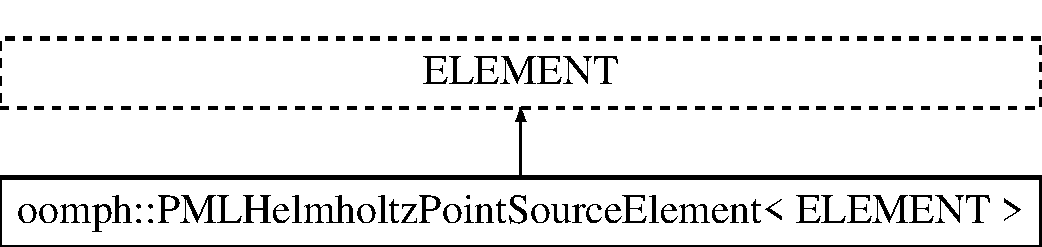
\includegraphics[height=2.000000cm]{classoomph_1_1PMLHelmholtzPointSourceElement}
\end{center}
\end{figure}
\subsection*{Public Member Functions}
\begin{DoxyCompactItemize}
\item 
\hyperlink{classoomph_1_1PMLHelmholtzPointSourceElement_a0092ffd22a364d8d4cb9013880a0d35b}{P\+M\+L\+Helmholtz\+Point\+Source\+Element} ()
\begin{DoxyCompactList}\small\item\em Constructor. \end{DoxyCompactList}\item 
\hyperlink{classoomph_1_1PMLHelmholtzPointSourceElement_a2d2f0c6620a08ce57dce4a5ee97fc079}{$\sim$\+P\+M\+L\+Helmholtz\+Point\+Source\+Element} ()
\begin{DoxyCompactList}\small\item\em Destructor (empty) \end{DoxyCompactList}\item 
void \hyperlink{classoomph_1_1PMLHelmholtzPointSourceElement_ad8a39b19e2387c97d46dd656f54e4cda}{setup} (const Vector$<$ double $>$ \&s\+\_\+point\+\_\+source, const std\+::complex$<$ double $>$ \&magnitude)
\begin{DoxyCompactList}\small\item\em Set local coordinate and magnitude of point source. \end{DoxyCompactList}\item 
void \hyperlink{classoomph_1_1PMLHelmholtzPointSourceElement_aa35993cf40bb93086076247797653397}{fill\+\_\+in\+\_\+contribution\+\_\+to\+\_\+residuals} (Vector$<$ double $>$ \&residuals)
\begin{DoxyCompactList}\small\item\em Add the element\textquotesingle{}s contribution to its residual vector (wrapper) \end{DoxyCompactList}\item 
void \hyperlink{classoomph_1_1PMLHelmholtzPointSourceElement_a046f79e3e1dcb266027366324e1e956d}{fill\+\_\+in\+\_\+contribution\+\_\+to\+\_\+jacobian} (Vector$<$ double $>$ \&residuals, Dense\+Matrix$<$ double $>$ \&jacobian)
\begin{DoxyCompactList}\small\item\em Add the element\textquotesingle{}s contribution to its residual vector and element Jacobian matrix (wrapper) \end{DoxyCompactList}\end{DoxyCompactItemize}
\subsection*{Private Member Functions}
\begin{DoxyCompactItemize}
\item 
void \hyperlink{classoomph_1_1PMLHelmholtzPointSourceElement_a3c9a152c82821bc163e0764125efd6d6}{fill\+\_\+in\+\_\+point\+\_\+source\+\_\+contribution\+\_\+to\+\_\+residuals} (Vector$<$ double $>$ \&residuals)
\begin{DoxyCompactList}\small\item\em Add the point source contribution to the residual vector. \end{DoxyCompactList}\end{DoxyCompactItemize}
\subsection*{Private Attributes}
\begin{DoxyCompactItemize}
\item 
Vector$<$ double $>$ \hyperlink{classoomph_1_1PMLHelmholtzPointSourceElement_afd6460c2714c0e00a078ab015cc8eb15}{S\+\_\+point\+\_\+source}
\begin{DoxyCompactList}\small\item\em Local coordinates of point at which point source is applied. \end{DoxyCompactList}\item 
std\+::complex$<$ double $>$ \hyperlink{classoomph_1_1PMLHelmholtzPointSourceElement_a64e3e8f4e30588c06ac79e69f1d02eb2}{Point\+\_\+source\+\_\+magnitude}
\begin{DoxyCompactList}\small\item\em Magnitude of point source (complex!) \end{DoxyCompactList}\end{DoxyCompactItemize}


\subsection{Detailed Description}
\subsubsection*{template$<$class E\+L\+E\+M\+E\+NT$>$\newline
class oomph\+::\+P\+M\+L\+Helmholtz\+Point\+Source\+Element$<$ E\+L\+E\+M\+E\+N\+T $>$}

Class to impose point source to (wrapped) Helmholtz element. 

Definition at line 233 of file oscillating\+\_\+sphere.\+cc.



\subsection{Constructor \& Destructor Documentation}
\mbox{\Hypertarget{classoomph_1_1PMLHelmholtzPointSourceElement_a0092ffd22a364d8d4cb9013880a0d35b}\label{classoomph_1_1PMLHelmholtzPointSourceElement_a0092ffd22a364d8d4cb9013880a0d35b}} 
\index{oomph\+::\+P\+M\+L\+Helmholtz\+Point\+Source\+Element@{oomph\+::\+P\+M\+L\+Helmholtz\+Point\+Source\+Element}!P\+M\+L\+Helmholtz\+Point\+Source\+Element@{P\+M\+L\+Helmholtz\+Point\+Source\+Element}}
\index{P\+M\+L\+Helmholtz\+Point\+Source\+Element@{P\+M\+L\+Helmholtz\+Point\+Source\+Element}!oomph\+::\+P\+M\+L\+Helmholtz\+Point\+Source\+Element@{oomph\+::\+P\+M\+L\+Helmholtz\+Point\+Source\+Element}}
\subsubsection{\texorpdfstring{P\+M\+L\+Helmholtz\+Point\+Source\+Element()}{PMLHelmholtzPointSourceElement()}}
{\footnotesize\ttfamily template$<$class E\+L\+E\+M\+E\+NT $>$ \\
\hyperlink{classoomph_1_1PMLHelmholtzPointSourceElement}{oomph\+::\+P\+M\+L\+Helmholtz\+Point\+Source\+Element}$<$ E\+L\+E\+M\+E\+NT $>$\+::\hyperlink{classoomph_1_1PMLHelmholtzPointSourceElement}{P\+M\+L\+Helmholtz\+Point\+Source\+Element} (\begin{DoxyParamCaption}{ }\end{DoxyParamCaption})\hspace{0.3cm}{\ttfamily [inline]}}



Constructor. 



Definition at line 239 of file oscillating\+\_\+sphere.\+cc.

\mbox{\Hypertarget{classoomph_1_1PMLHelmholtzPointSourceElement_a2d2f0c6620a08ce57dce4a5ee97fc079}\label{classoomph_1_1PMLHelmholtzPointSourceElement_a2d2f0c6620a08ce57dce4a5ee97fc079}} 
\index{oomph\+::\+P\+M\+L\+Helmholtz\+Point\+Source\+Element@{oomph\+::\+P\+M\+L\+Helmholtz\+Point\+Source\+Element}!````~P\+M\+L\+Helmholtz\+Point\+Source\+Element@{$\sim$\+P\+M\+L\+Helmholtz\+Point\+Source\+Element}}
\index{````~P\+M\+L\+Helmholtz\+Point\+Source\+Element@{$\sim$\+P\+M\+L\+Helmholtz\+Point\+Source\+Element}!oomph\+::\+P\+M\+L\+Helmholtz\+Point\+Source\+Element@{oomph\+::\+P\+M\+L\+Helmholtz\+Point\+Source\+Element}}
\subsubsection{\texorpdfstring{$\sim$\+P\+M\+L\+Helmholtz\+Point\+Source\+Element()}{~PMLHelmholtzPointSourceElement()}}
{\footnotesize\ttfamily template$<$class E\+L\+E\+M\+E\+NT $>$ \\
\hyperlink{classoomph_1_1PMLHelmholtzPointSourceElement}{oomph\+::\+P\+M\+L\+Helmholtz\+Point\+Source\+Element}$<$ E\+L\+E\+M\+E\+NT $>$\+::$\sim$\hyperlink{classoomph_1_1PMLHelmholtzPointSourceElement}{P\+M\+L\+Helmholtz\+Point\+Source\+Element} (\begin{DoxyParamCaption}{ }\end{DoxyParamCaption})\hspace{0.3cm}{\ttfamily [inline]}}



Destructor (empty) 



Definition at line 246 of file oscillating\+\_\+sphere.\+cc.



\subsection{Member Function Documentation}
\mbox{\Hypertarget{classoomph_1_1PMLHelmholtzPointSourceElement_a046f79e3e1dcb266027366324e1e956d}\label{classoomph_1_1PMLHelmholtzPointSourceElement_a046f79e3e1dcb266027366324e1e956d}} 
\index{oomph\+::\+P\+M\+L\+Helmholtz\+Point\+Source\+Element@{oomph\+::\+P\+M\+L\+Helmholtz\+Point\+Source\+Element}!fill\+\_\+in\+\_\+contribution\+\_\+to\+\_\+jacobian@{fill\+\_\+in\+\_\+contribution\+\_\+to\+\_\+jacobian}}
\index{fill\+\_\+in\+\_\+contribution\+\_\+to\+\_\+jacobian@{fill\+\_\+in\+\_\+contribution\+\_\+to\+\_\+jacobian}!oomph\+::\+P\+M\+L\+Helmholtz\+Point\+Source\+Element@{oomph\+::\+P\+M\+L\+Helmholtz\+Point\+Source\+Element}}
\subsubsection{\texorpdfstring{fill\+\_\+in\+\_\+contribution\+\_\+to\+\_\+jacobian()}{fill\_in\_contribution\_to\_jacobian()}}
{\footnotesize\ttfamily template$<$class E\+L\+E\+M\+E\+NT $>$ \\
void \hyperlink{classoomph_1_1PMLHelmholtzPointSourceElement}{oomph\+::\+P\+M\+L\+Helmholtz\+Point\+Source\+Element}$<$ E\+L\+E\+M\+E\+NT $>$\+::fill\+\_\+in\+\_\+contribution\+\_\+to\+\_\+jacobian (\begin{DoxyParamCaption}\item[{Vector$<$ double $>$ \&}]{residuals,  }\item[{Dense\+Matrix$<$ double $>$ \&}]{jacobian }\end{DoxyParamCaption})\hspace{0.3cm}{\ttfamily [inline]}}



Add the element\textquotesingle{}s contribution to its residual vector and element Jacobian matrix (wrapper) 



Definition at line 272 of file oscillating\+\_\+sphere.\+cc.

\mbox{\Hypertarget{classoomph_1_1PMLHelmholtzPointSourceElement_aa35993cf40bb93086076247797653397}\label{classoomph_1_1PMLHelmholtzPointSourceElement_aa35993cf40bb93086076247797653397}} 
\index{oomph\+::\+P\+M\+L\+Helmholtz\+Point\+Source\+Element@{oomph\+::\+P\+M\+L\+Helmholtz\+Point\+Source\+Element}!fill\+\_\+in\+\_\+contribution\+\_\+to\+\_\+residuals@{fill\+\_\+in\+\_\+contribution\+\_\+to\+\_\+residuals}}
\index{fill\+\_\+in\+\_\+contribution\+\_\+to\+\_\+residuals@{fill\+\_\+in\+\_\+contribution\+\_\+to\+\_\+residuals}!oomph\+::\+P\+M\+L\+Helmholtz\+Point\+Source\+Element@{oomph\+::\+P\+M\+L\+Helmholtz\+Point\+Source\+Element}}
\subsubsection{\texorpdfstring{fill\+\_\+in\+\_\+contribution\+\_\+to\+\_\+residuals()}{fill\_in\_contribution\_to\_residuals()}}
{\footnotesize\ttfamily template$<$class E\+L\+E\+M\+E\+NT $>$ \\
void \hyperlink{classoomph_1_1PMLHelmholtzPointSourceElement}{oomph\+::\+P\+M\+L\+Helmholtz\+Point\+Source\+Element}$<$ E\+L\+E\+M\+E\+NT $>$\+::fill\+\_\+in\+\_\+contribution\+\_\+to\+\_\+residuals (\begin{DoxyParamCaption}\item[{Vector$<$ double $>$ \&}]{residuals }\end{DoxyParamCaption})\hspace{0.3cm}{\ttfamily [inline]}}



Add the element\textquotesingle{}s contribution to its residual vector (wrapper) 



Definition at line 258 of file oscillating\+\_\+sphere.\+cc.

\mbox{\Hypertarget{classoomph_1_1PMLHelmholtzPointSourceElement_a3c9a152c82821bc163e0764125efd6d6}\label{classoomph_1_1PMLHelmholtzPointSourceElement_a3c9a152c82821bc163e0764125efd6d6}} 
\index{oomph\+::\+P\+M\+L\+Helmholtz\+Point\+Source\+Element@{oomph\+::\+P\+M\+L\+Helmholtz\+Point\+Source\+Element}!fill\+\_\+in\+\_\+point\+\_\+source\+\_\+contribution\+\_\+to\+\_\+residuals@{fill\+\_\+in\+\_\+point\+\_\+source\+\_\+contribution\+\_\+to\+\_\+residuals}}
\index{fill\+\_\+in\+\_\+point\+\_\+source\+\_\+contribution\+\_\+to\+\_\+residuals@{fill\+\_\+in\+\_\+point\+\_\+source\+\_\+contribution\+\_\+to\+\_\+residuals}!oomph\+::\+P\+M\+L\+Helmholtz\+Point\+Source\+Element@{oomph\+::\+P\+M\+L\+Helmholtz\+Point\+Source\+Element}}
\subsubsection{\texorpdfstring{fill\+\_\+in\+\_\+point\+\_\+source\+\_\+contribution\+\_\+to\+\_\+residuals()}{fill\_in\_point\_source\_contribution\_to\_residuals()}}
{\footnotesize\ttfamily template$<$class E\+L\+E\+M\+E\+NT $>$ \\
void \hyperlink{classoomph_1_1PMLHelmholtzPointSourceElement}{oomph\+::\+P\+M\+L\+Helmholtz\+Point\+Source\+Element}$<$ E\+L\+E\+M\+E\+NT $>$\+::fill\+\_\+in\+\_\+point\+\_\+source\+\_\+contribution\+\_\+to\+\_\+residuals (\begin{DoxyParamCaption}\item[{Vector$<$ double $>$ \&}]{residuals }\end{DoxyParamCaption})\hspace{0.3cm}{\ttfamily [inline]}, {\ttfamily [private]}}



Add the point source contribution to the residual vector. 



Definition at line 288 of file oscillating\+\_\+sphere.\+cc.

\mbox{\Hypertarget{classoomph_1_1PMLHelmholtzPointSourceElement_ad8a39b19e2387c97d46dd656f54e4cda}\label{classoomph_1_1PMLHelmholtzPointSourceElement_ad8a39b19e2387c97d46dd656f54e4cda}} 
\index{oomph\+::\+P\+M\+L\+Helmholtz\+Point\+Source\+Element@{oomph\+::\+P\+M\+L\+Helmholtz\+Point\+Source\+Element}!setup@{setup}}
\index{setup@{setup}!oomph\+::\+P\+M\+L\+Helmholtz\+Point\+Source\+Element@{oomph\+::\+P\+M\+L\+Helmholtz\+Point\+Source\+Element}}
\subsubsection{\texorpdfstring{setup()}{setup()}}
{\footnotesize\ttfamily template$<$class E\+L\+E\+M\+E\+NT $>$ \\
void \hyperlink{classoomph_1_1PMLHelmholtzPointSourceElement}{oomph\+::\+P\+M\+L\+Helmholtz\+Point\+Source\+Element}$<$ E\+L\+E\+M\+E\+NT $>$\+::setup (\begin{DoxyParamCaption}\item[{const Vector$<$ double $>$ \&}]{s\+\_\+point\+\_\+source,  }\item[{const std\+::complex$<$ double $>$ \&}]{magnitude }\end{DoxyParamCaption})\hspace{0.3cm}{\ttfamily [inline]}}



Set local coordinate and magnitude of point source. 



Definition at line 249 of file oscillating\+\_\+sphere.\+cc.



\subsection{Member Data Documentation}
\mbox{\Hypertarget{classoomph_1_1PMLHelmholtzPointSourceElement_a64e3e8f4e30588c06ac79e69f1d02eb2}\label{classoomph_1_1PMLHelmholtzPointSourceElement_a64e3e8f4e30588c06ac79e69f1d02eb2}} 
\index{oomph\+::\+P\+M\+L\+Helmholtz\+Point\+Source\+Element@{oomph\+::\+P\+M\+L\+Helmholtz\+Point\+Source\+Element}!Point\+\_\+source\+\_\+magnitude@{Point\+\_\+source\+\_\+magnitude}}
\index{Point\+\_\+source\+\_\+magnitude@{Point\+\_\+source\+\_\+magnitude}!oomph\+::\+P\+M\+L\+Helmholtz\+Point\+Source\+Element@{oomph\+::\+P\+M\+L\+Helmholtz\+Point\+Source\+Element}}
\subsubsection{\texorpdfstring{Point\+\_\+source\+\_\+magnitude}{Point\_source\_magnitude}}
{\footnotesize\ttfamily template$<$class E\+L\+E\+M\+E\+NT $>$ \\
std\+::complex$<$double$>$ \hyperlink{classoomph_1_1PMLHelmholtzPointSourceElement}{oomph\+::\+P\+M\+L\+Helmholtz\+Point\+Source\+Element}$<$ E\+L\+E\+M\+E\+NT $>$\+::Point\+\_\+source\+\_\+magnitude\hspace{0.3cm}{\ttfamily [private]}}



Magnitude of point source (complex!) 



Definition at line 347 of file oscillating\+\_\+sphere.\+cc.

\mbox{\Hypertarget{classoomph_1_1PMLHelmholtzPointSourceElement_afd6460c2714c0e00a078ab015cc8eb15}\label{classoomph_1_1PMLHelmholtzPointSourceElement_afd6460c2714c0e00a078ab015cc8eb15}} 
\index{oomph\+::\+P\+M\+L\+Helmholtz\+Point\+Source\+Element@{oomph\+::\+P\+M\+L\+Helmholtz\+Point\+Source\+Element}!S\+\_\+point\+\_\+source@{S\+\_\+point\+\_\+source}}
\index{S\+\_\+point\+\_\+source@{S\+\_\+point\+\_\+source}!oomph\+::\+P\+M\+L\+Helmholtz\+Point\+Source\+Element@{oomph\+::\+P\+M\+L\+Helmholtz\+Point\+Source\+Element}}
\subsubsection{\texorpdfstring{S\+\_\+point\+\_\+source}{S\_point\_source}}
{\footnotesize\ttfamily template$<$class E\+L\+E\+M\+E\+NT $>$ \\
Vector$<$double$>$ \hyperlink{classoomph_1_1PMLHelmholtzPointSourceElement}{oomph\+::\+P\+M\+L\+Helmholtz\+Point\+Source\+Element}$<$ E\+L\+E\+M\+E\+NT $>$\+::S\+\_\+point\+\_\+source\hspace{0.3cm}{\ttfamily [private]}}



Local coordinates of point at which point source is applied. 



Definition at line 344 of file oscillating\+\_\+sphere.\+cc.



The documentation for this class was generated from the following file\+:\begin{DoxyCompactItemize}
\item 
\hyperlink{oscillating__sphere_8cc}{oscillating\+\_\+sphere.\+cc}\end{DoxyCompactItemize}

\chapter{File Documentation}
\hypertarget{oscillating__sphere_8cc}{}\section{oscillating\+\_\+sphere.\+cc File Reference}
\label{oscillating__sphere_8cc}\index{oscillating\+\_\+sphere.\+cc@{oscillating\+\_\+sphere.\+cc}}
\subsection*{Classes}
\begin{DoxyCompactItemize}
\item 
class \hyperlink{classoomph_1_1PMLHelmholtzPointSourceElement}{oomph\+::\+P\+M\+L\+Helmholtz\+Point\+Source\+Element$<$ E\+L\+E\+M\+E\+N\+T $>$}
\begin{DoxyCompactList}\small\item\em Class to impose point source to (wrapped) Helmholtz element. \end{DoxyCompactList}\item 
class \hyperlink{classoomph_1_1FaceGeometry_3_01PMLHelmholtzPointSourceElement_3_01ELEMENT_01_4_01_4}{oomph\+::\+Face\+Geometry$<$ P\+M\+L\+Helmholtz\+Point\+Source\+Element$<$ E\+L\+E\+M\+E\+N\+T $>$ $>$}
\item 
class \hyperlink{classoomph_1_1FaceGeometry_3_01FaceGeometry_3_01PMLHelmholtzPointSourceElement_3_01ELEMENT_01_4_01_4_01_4}{oomph\+::\+Face\+Geometry$<$ Face\+Geometry$<$ P\+M\+L\+Helmholtz\+Point\+Source\+Element$<$ E\+L\+E\+M\+E\+N\+T $>$ $>$ $>$}
\item 
class \hyperlink{classoomph_1_1EquivalentQElement_3_01PMLHelmholtzPointSourceElement_3_01ELEMENT_01_4_01_4}{oomph\+::\+Equivalent\+Q\+Element$<$ P\+M\+L\+Helmholtz\+Point\+Source\+Element$<$ E\+L\+E\+M\+E\+N\+T $>$ $>$}
\item 
class \hyperlink{classoomph_1_1EquivalentQElement_3_01ProjectablePMLFourierDecomposedHelmholtzElement_3_01PMLHelmea655fba41d5fa485ebddcd1b3c02e7e}{oomph\+::\+Equivalent\+Q\+Element$<$ Projectable\+P\+M\+L\+Fourier\+Decomposed\+Helmholtz\+Element$<$ P\+M\+L\+Helmholtz\+Point\+Source\+Element$<$ E\+L\+E\+M\+E\+N\+T $>$ $>$ $>$}
\item 
class \hyperlink{classPMLFourierDecomposedHelmholtzProblem}{P\+M\+L\+Fourier\+Decomposed\+Helmholtz\+Problem$<$ E\+L\+E\+M\+E\+N\+T $>$}
\begin{DoxyCompactList}\small\item\em Problem class. \end{DoxyCompactList}\end{DoxyCompactItemize}
\subsection*{Namespaces}
\begin{DoxyCompactItemize}
\item 
 \hyperlink{namespaceProblemParameters}{Problem\+Parameters}
\begin{DoxyCompactList}\small\item\em Namespace for the Fourier decomposed Helmholtz problem parameters. \end{DoxyCompactList}\item 
 \hyperlink{namespaceoomph}{oomph}
\end{DoxyCompactItemize}
\subsection*{Functions}
\begin{DoxyCompactItemize}
\item 
Vector$<$ double $>$ \hyperlink{namespaceProblemParameters_a20cc9776e745842f6126f4cd17659d19}{Problem\+Parameters\+::\+Coeff} (N\+\_\+terms, 1.\+0)
\begin{DoxyCompactList}\small\item\em Coefficients in the exact solution. \end{DoxyCompactList}\item 
std\+::complex$<$ double $>$ \hyperlink{namespaceProblemParameters_a869b19d379dd66b387c675ca07c6a049}{Problem\+Parameters\+::I} (0.\+0, 1.\+0)
\begin{DoxyCompactList}\small\item\em Imaginary unit. \end{DoxyCompactList}\item 
void \hyperlink{namespaceProblemParameters_af750b29069b29bd38b5220ecf534e7f7}{Problem\+Parameters\+::get\+\_\+exact\+\_\+u} (const Vector$<$ double $>$ \&x, Vector$<$ double $>$ \&u)
\begin{DoxyCompactList}\small\item\em Exact solution as a Vector of size 2, containing real and imag parts. \end{DoxyCompactList}\item 
void \hyperlink{namespaceProblemParameters_aa544d1f3e384d3283f7113512931ea8f}{Problem\+Parameters\+::exact\+\_\+minus\+\_\+dudr} (const Vector$<$ double $>$ \&x, std\+::complex$<$ double $>$ \&flux)
\begin{DoxyCompactList}\small\item\em Get -\/du/dr (spherical r) for exact solution. Equal to prescribed flux on inner boundary. \end{DoxyCompactList}\item 
std\+::complex$<$ double $>$ \hyperlink{namespaceProblemParameters_acdaa2237a50d2ccf2b58be59c944953d}{Problem\+Parameters\+::\+Magnitude} (100.\+0, 100.\+0)
\begin{DoxyCompactList}\small\item\em Point source magnitude (Complex) \end{DoxyCompactList}\item 
int \hyperlink{oscillating__sphere_8cc_a3c04138a5bfe5d72780bb7e82a18e627}{main} (int argc, char $\ast$$\ast$argv)
\begin{DoxyCompactList}\small\item\em Driver code for Pml Fourier decomposed Helmholtz problem. \end{DoxyCompactList}\end{DoxyCompactItemize}
\subsection*{Variables}
\begin{DoxyCompactItemize}
\item 
string \hyperlink{namespaceProblemParameters_a9df0f1728e8e7e53dcca84385ae9a031}{Problem\+Parameters\+::\+Directory} =\char`\"{}R\+E\+S\+LT\char`\"{}
\begin{DoxyCompactList}\small\item\em Output directory. \end{DoxyCompactList}\item 
double \hyperlink{namespaceProblemParameters_aa5362de1af9e257fde4317c367158a93}{Problem\+Parameters\+::\+K\+\_\+squared} = 10.\+0
\begin{DoxyCompactList}\small\item\em Frequency. \end{DoxyCompactList}\item 
double \hyperlink{namespaceProblemParameters_ad56d4d5946cbe68de28413e4f8aa4d42}{Problem\+Parameters\+::\+P\+M\+L\+\_\+thickness} =4.\+0
\begin{DoxyCompactList}\small\item\em Default physical P\+ML thickness. \end{DoxyCompactList}\item 
unsigned \hyperlink{namespaceProblemParameters_aef2e7cb819b8c5012a0f2db03892ee87}{Problem\+Parameters\+::\+Nel\+\_\+pml} =15
\begin{DoxyCompactList}\small\item\em Default number of elements within P\+M\+Ls. \end{DoxyCompactList}\item 
double \hyperlink{namespaceProblemParameters_aafe26abadfce87800a6a4676f0476956}{Problem\+Parameters\+::\+Element\+\_\+area} = 0.\+1
\begin{DoxyCompactList}\small\item\em Target area for initial mesh. \end{DoxyCompactList}\item 
int \hyperlink{namespaceProblemParameters_aaa674958a1ca6ee0b99de3377288c93f}{Problem\+Parameters\+::\+N\+\_\+fourier} =0
\begin{DoxyCompactList}\small\item\em The default Fourier wave number. \end{DoxyCompactList}\item 
unsigned \hyperlink{namespaceProblemParameters_a6361f0f1c4a120e62d28db64baa84b40}{Problem\+Parameters\+::\+N\+\_\+terms} =6
\begin{DoxyCompactList}\small\item\em Number of terms in the exact solution. \end{DoxyCompactList}\item 
double \hyperlink{namespaceProblemParameters_a42c148c7f3bed95827acf8d86c2c6089}{Problem\+Parameters\+::\+R\+\_\+source} = 2.\+0
\begin{DoxyCompactList}\small\item\em Radial position of point source. \end{DoxyCompactList}\item 
double \hyperlink{namespaceProblemParameters_a346993de7a274e1828af3f8fc8ca8b13}{Problem\+Parameters\+::\+Z\+\_\+source} = 2.\+0
\begin{DoxyCompactList}\small\item\em Axial position of point source. \end{DoxyCompactList}\end{DoxyCompactItemize}


\subsection{Function Documentation}
\mbox{\Hypertarget{oscillating__sphere_8cc_a3c04138a5bfe5d72780bb7e82a18e627}\label{oscillating__sphere_8cc_a3c04138a5bfe5d72780bb7e82a18e627}} 
\index{oscillating\+\_\+sphere.\+cc@{oscillating\+\_\+sphere.\+cc}!main@{main}}
\index{main@{main}!oscillating\+\_\+sphere.\+cc@{oscillating\+\_\+sphere.\+cc}}
\subsubsection{\texorpdfstring{main()}{main()}}
{\footnotesize\ttfamily int main (\begin{DoxyParamCaption}\item[{int}]{argc,  }\item[{char $\ast$$\ast$}]{argv }\end{DoxyParamCaption})}



Driver code for Pml Fourier decomposed Helmholtz problem. 



Definition at line 1188 of file oscillating\+\_\+sphere.\+cc.



References Problem\+Parameters\+::\+Directory, Problem\+Parameters\+::\+Element\+\_\+area, Problem\+Parameters\+::\+K\+\_\+squared, Problem\+Parameters\+::\+N\+\_\+fourier, Problem\+Parameters\+::\+Nel\+\_\+pml, and Problem\+Parameters\+::\+P\+M\+L\+\_\+thickness.


\hypertarget{oscillating__sphere_8txt__doxygenified_8h}{}\section{oscillating\+\_\+sphere.\+txt\+\_\+doxygenified.\+h File Reference}
\label{oscillating__sphere_8txt__doxygenified_8h}\index{oscillating\+\_\+sphere.\+txt\+\_\+doxygenified.\+h@{oscillating\+\_\+sphere.\+txt\+\_\+doxygenified.\+h}}

%--- End generated contents ---

% Index
\backmatter
\newpage
\phantomsection
\clearemptydoublepage
\addcontentsline{toc}{chapter}{Index}
\printindex

\end{document}
